\section{Pourquoi utiliser un moteur à gaz ?}

	L’utilisation de l’air comme fluide moteur, plutôt que la vapeur, apporte plusieurs avantages.

	\begin{itemize}
		\item D’une part, il est possible de se dispenser entièrement des condenseurs et refroidisseurs. La phase de refroidissement (\S\ref{ch_demo_second_principe}) a lieu directement dans l’atmosphère, qui accueille aisément tous les gaz chauds que l’on rejette, et qui sert de réservoir dans lequel puiser de l’air frais pour réalimenter le moteur.

		À puissance égale, la masse, le volume et souvent le coût des moteurs à gaz sont donc très fortement réduits par rapport à leurs homologues à vapeur. Ceci est particulièrement intéressant lorsque le moteur doit participer à la portée de son propre poids.

		\item D’autre part, l’apport de chaleur se fait sans perte. En effet, il est possible d’effectuer une combustion \emph{directement à l’intérieur} du fluide de travail --\ c’est ce que l’on nomme la \vocab{combustion interne}.

		Alors que les installations à vapeur laissent s’échapper de grandes quantités de chaleur au-dessus de la chaudière (\S\ref{ch_chaudière}), les moteurs à air perdent très peu de chaleur dans les phases de combustion.
	\end{itemize}

	Le principal défaut des moteurs à gaz est que la combustion interne impose une qualité de carburant élevée. Les résidus de combustion devant circuler à l’intérieur même de la partie thermodynamique de la machine, nous ne pouvons utiliser des sources de chaleur intéressantes ou économiques telles que la combustion des déchets, du bois, ou même du charbon.

	Au final, la légèreté relative des moteurs à air par rapport à leurs homologues à vapeur fait qu’ils sont systématiquement utilisés lorsque la masse joue un rôle important, comme dans les transports aériens ou routiers.



\section{Critères d’évaluation des moteurs à gaz}
\label{ch_criteres_evaluation_moteurs_gaz}

	\subsection{Le rendement thermique}

		Il va désormais de soi que nous cherchons toujours à obtenir une grande \vocab{efficacité thermique} $\eta_\text{moteur} \equiv \left| \frac{\dot{W}_\net}{\dot{Q}_\inn} \right|$ (\ref{def_rendement_moteur}) en gardant à l’esprit qu’elle ne peut excéder son maximum théorique $\eta _{moteur Carnot} = 1 - \frac{T_\text{min.}}{T_\text{max.}}$ (\ref{eq_efficacité_moteur_carnot_température}).

		Comme nous l’avons déjà suggéré en \S\ref{ch_evaluation_moteurs_vapeur}, le rendement thermique ne doit toutefois pas être maximisé au détriment d’autres paramètres importants, dont nous présentons plus bas les plus notables pour les moteurs à gaz.

	\subsection{La marge de travail}
	\label{ch_rapport_des_puissances}

		Dans un moteur en fonctionnement, l’irréversibilité des compressions et détentes n’est pas indépendante de la vitesse. Lorsqu’ils fonctionnent hors de leur plage de fonctionnement optimale, les moteurs voient ainsi leur puissance spécifique diminuer. Les irréversibilités peuvent même réduire le rendement à zéro, le moteur tournant alors sans produire de travail utile (exactement comme un moteur automobile débrayé). La \vocab{marge de travail} est un concept qui permet d’évaluer la robustesse d’un cycle à l’augmentation de ces irréversibilités.

		Pour aborder ce concept, étudions premièrement le cas d’un moteur dont la compression et la détente sont réversibles. Les transferts énergétiques du cycle sont décrits en \cref{fig_rapport_puissances_1}. Si au lieu d’être idéale, la turbine de ce premier moteur se voyait soudainement affublée d’un rendement isentropique de~\SI{95}{\percent}, elle ne fournirait plus que \SI{95}{\watt}. La puissance effective du moteur passerait alors de~\num{10}~à~\SI{5}{\watt} --\ une réduction de~\SI{50}{\percent}.

		\begin{figure}%FIXME : vérifier l’acceptabilité / le seuil d’originalité de cette figure, qui est probablement repiquée de Çengel et al
			\begin{center}
				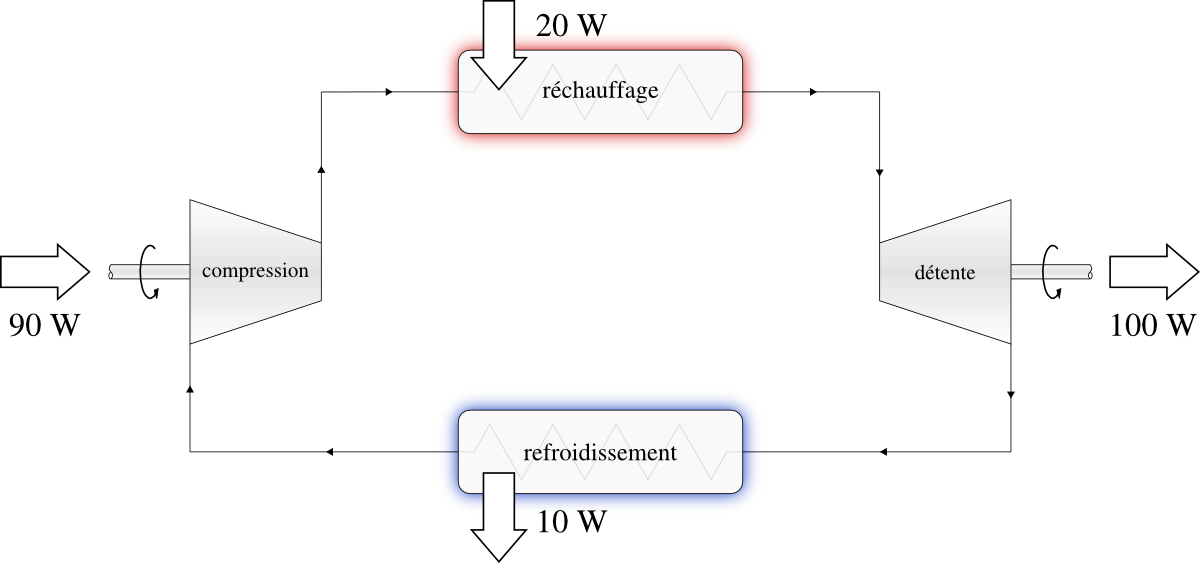
\includegraphics[width=\textwidth]{images/marge_travail_1.png}
			\end{center}
			\supercaption{Le cycle d’un moteur (hypothétique) à faible marge de travail. La puissance développée est de $\dot W_\net = \dot W_\text{compression} + \dot W_\text{détente} = \num{+90} + (\num{-100}) = \SI{-10}{\watt}$, et le rendement $\eta_\text{moteur} = -\frac{\dot W_\net}{\dot Q_\inn} = -\frac{\num{-10}}{\num{20}} = \SI{50}{\percent}$.}{schéma \cczero \oc}
			\label{fig_rapport_puissances_1}
		\end{figure}

		Comparons maintenant ce cas avec un moteur de même rendement, même puissance, mais dont le cycle est différent, comme montré en \cref{fig_rapport_puissances_2}. Dans ce moteur, si l’efficacité isentropique de la turbine passait de~\SI{100}{\percent} à~\SI{95}{\percent}, la puissance nette passerait de~10~à~\SI{9}{\watt} --\ une baisse de~\SI{10}{\percent} seulement.

		\begin{figure}%FIXME : vérifier l’acceptabilité / le seuil d’originalité de cette figure, qui est probablement repiquée de Çengel et al
			\begin{center}
				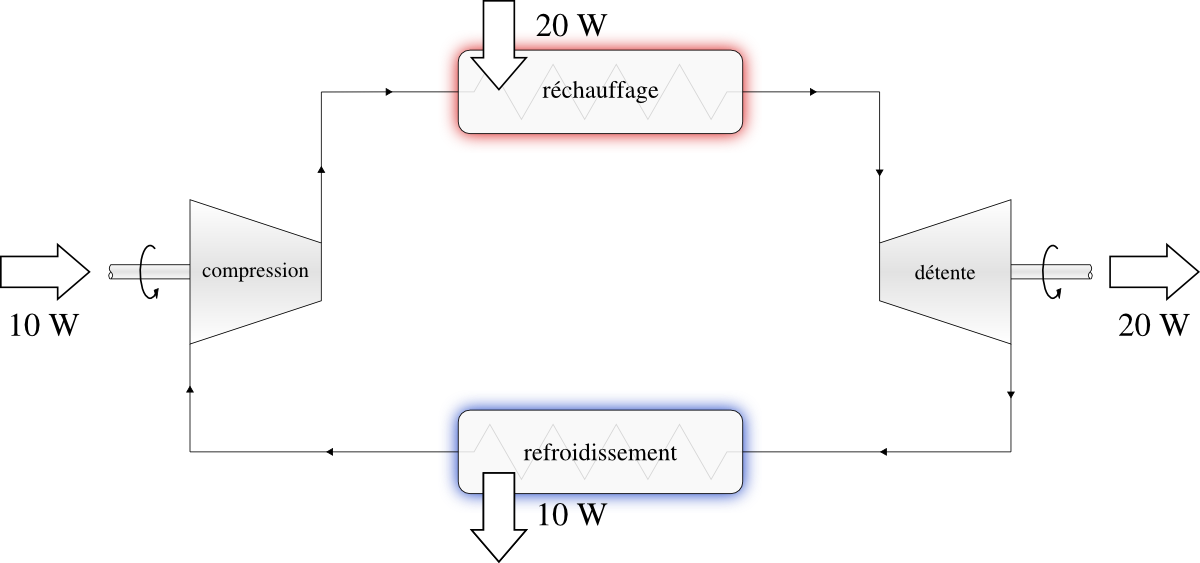
\includegraphics[width=\textwidth]{images/marge_travail_2.png}
			\end{center}
			\supercaption{Le cycle d’un second moteur (hypothétique), à forte marge de travail. La puissance développée $\dot W_\net = \num{+10} + (\num{-20}) = \SI{-10}{\watt}$, et le rendement $\eta_\text{moteur} = -\frac{\num{-10}}{\num{20}} = \SI{50}{\percent}$ sont identiques à celles du moteur décrit en \cref{fig_rapport_puissances_1}.}{schéma \cczero \oc}
			\label{fig_rapport_puissances_2}
		\end{figure}

		On peut ainsi voir que plus la part de la turbine dans la puissance nette développée est grande, moins l’efficacité du cycle est affectée par les irréversibilités. Nous généralisons et formalisons cela avec le concept de \vocab{marge de travail} $M_w$ (en anglais : \vocabe{work ratio}), défini comme le rapport entre la puissance nette et la puissance brute d’un moteur :
		\begin{equation}
			M_w \equiv 	\frac{\dot W_\net}{\dot W_\text{brut}}	= \frac{\dot W_\text{détentes} + \dot W_\text{compressions}}{\dot W_\text{détentes}}
			\label{eq_marge_travail}
		\end{equation}
		\begin{equationterms}
			\item où \tab $M_w$ 									\tab\tab\tab\tab\tab\tab\tab\tab est la marge de travail (sans unité) ;
			\item \tab $\dot W_\text{détentes}$ 			\tab\tab\tab\tab est la puissance dégagée pendant les détentes ;
			\item et \tab $\dot W_\text{compressions}$ 	\tab la puissance consommée lors des compressions.
		\end{equationterms}

		Une machine dont la marge de travail est grande perd moins de son efficacité lorsqu’elle fonctionne hors de sa plage de régime optimale : elle est donc plus souple d’utilisation. La marge de travail est l’un des indicateurs de la réactivité d’un moteur, c’est-à-dire de sa capacité à changer de puissance et de régime rapidement. On peut établir un parallèle avec la notion de \vocab{marge bénéficiaire nette} en économie : toutes choses égales par ailleurs, il est plus intéressant de commercialiser à \SI{3}{\euroo} des objets achetés \SI{2}{\euroo} pièce, qu’à \SI{101}{\euroo} des objets achetés \SI{100}{\euroo} pièce, notamment parce que le bénéfice de \SI{1}{\euroo} est alors moins sensible à une variation de prix ou de coût imposée par le marché.
		
			Le moteur de Carnot est l’exemple-type d’un cycle thermodynamique à haut rendement mais dont la marge de travail est très faible. En traçant le cycle sur un diagramme pression-volume (\cref{fig_p-v_gp_carnot}) cette faiblesse ressort bien : les courbes lors des phases de compression et détente sont très proches l’une de l’autre. Rankine, lorsqu’il modifie ce cycle (\S\ref{ch_cycle_de_rankine}), augmente considérablement la marge de travail.

		D’une façon générale, une grande efficacité thermique requiert un grand taux de compression (afin d’obtenir une haute température avant que le transfert de chaleur ne soit initié). Une grande marge de travail requiert un faible travail de compression (afin de minimiser la sensibilité du moteur aux irréversibilités). Ces deux objectifs sont donc souvent contradictoires et il reviendra à l’ingénieur/e thermodynamicien/ne de trouver le meilleur compromis.
		 

	\subsection{Poussée et puissance spécifiques}
	\label{ch_poussee_puissance_specifiques}

		Nous utilisons les concepts de \vocab{poussée spécifique} $\frac{P}{\dot m}$ et \vocab{puissance spécifique} $w_\net$, c’est-à-dire la poussée et la puissance du moteur divisées par le débit d’air qui le traverse, pour comparer sommairement les cycles moteurs entre eux. Il est souvent désirable d’augmenter ces paramètres dans les applications où un grand rapport puissance/poids est recherché.

		Ainsi par exemple, sur un moteur aéronautique, une augmentation du rendement n’est pas toujours justifiée si elle provoque une augmentation du poids ou de l’encombrement. Un aéronef plus lourd doit fournir une plus grande portance, ce qui augmente la traînée … et donc la poussée, et la puissance nécessaire pour la générer.

	
	\subsection{Autres critères d’évaluation}
	
		De nombreux autres critères sont naturellement à prendre en compte dans la conception d’un moteur, dont l’exploration dépasse le cadre de notre étude. Nous notons rapidement, entre autres :
		
		\begin{itemize}
			\item le coût d’achat, qui est directement lié à la complexité et à la taille du moteur ;
			\item l’impact écologique ;
			\item la facilité de maintenance et la fiabilité ;
			\item la réactivité ;
			\item le niveau de vibration engendré.
		\end{itemize}

		La prise en compte de chacun ces facteurs peut justifier de limiter sciemment l’efficacité du moteur. Nous ferons ainsi le pari que lors de l’acquisition de son premier véhicule, l’étudiant/e attachera plus d’importance au coût d’achat qu’à la consommation de carburant --\ de même qu’il/\-elle n’optera pas pour une motorisation de compétition nécessitant une maintenance incessante.
		
		À vrai dire, il y a bien peu à ajouter à ce qu’expliquait déjà notre émérite et favori théoricien en 1824 :

		\begin{quote}
			On ne doit pas se flatter de mettre jamais à profit, dans la pratique, toute la puissance motrice des combustibles. Les tentatives que l’on ferait pour approcher de ce résultat seraient même plus nuisibles qu’utiles, si elles faisaient négliger d’autres considérations importantes. L’économie du combustible n’est qu’une des conditions à remplir par les machines à feu ; dans beaucoup de circonstances, elle n’est que secondaire, elle doit souvent céder le pas à la sûreté, à la solidité, à la durée de la machine, au peu de place qu’il faut lui faire occuper, au peu de frais de son établissement, etc. Savoir apprécier, dans chaque cas, à leur juste valeur, les considérations de convenance et d’économie qui peuvent se présenter, savoir discerner les plus importantes de celles qui sont seulement accessoires, les balancer toutes convenablement entre elles, afin de parvenir par les moyens les plus faciles au meilleur résultat, tel doit être le principal talent de l’homme [ou de la femme] appelé à diriger, à coordonner entre eux les travaux de ses semblables, à les faire concourir vers un but utile de quelque genre qu’il soit.
			\begin{flushright}
				Sadi Carnot, 1824~\cite{carnot1824}
			\end{flushright}
		\end{quote}



\section{Moteurs alternatifs}

Les moteurs à mouvement alternatif (souvent dits «~à pistons-cylindres~») admettent une quantité d’air finie et effectuent leur cycle thermodynamique sur cette masse. Le cycle peut être effectué de multiples fois en parallèle, et est répété plusieurs fois dans le temps pour fournir une puissance continue (un moteur automobile effectue usuellement une cinquantaine de cycles par seconde).

	\subsection{Intérêt des moteurs à pistons}

		D’un point de vue thermodynamique, le principal avantage de ces moteurs est que la manipulation d’une masse fixe d’air est beaucoup plus aisée que celle d’un flux continu. Il est possible, par exemple, d’effectuer une combustion à température constante (telle que le préconise Carnot) en faisant varier le volume pendant la combustion. La même opération en régime continu requerrait que la combustion s’effectue au sein d’une turbine, ce que l’on ne sait pas encore faire à échelle industrielle.

		Un second avantage des moteurs à pistons est que la température maximale du cycle n’y est atteinte que sporadiquement (périodiquement, mais toujours brièvement). Il est ainsi possible, lors de la combustion, de faire atteindre au gaz des températures qui dépassent les limites métallurgiques du moteur, avec les avantages pour le rendement que nous avons abordés au \courssept.

		Le poids et la complexité de leurs mécanismes (bielles, vilebrequin, soupapes, circuits divers), en revanche, défavorisent les moteurs à pistons lorsque de très grandes puissances et vitesses de rotation sont requises.


	\subsection{Le cycle d’Otto}
	
		On doit à l’ingénieur allemand \wf{Nikolaus Otto}, en 1864, la mise au point du moteur que l’on connaît aujourd’hui sous le nom de «~\vocab{moteur à essence}~». Le cycle de principe de ce moteur, appelé \vocab{cycle d’Otto}, est constitué de deux phases isentropiques encadrées par deux phases isochores ; il est décrit en \cref{fig_cycle_otto}. 
		
		\begin{figure}
			\begin{center}
				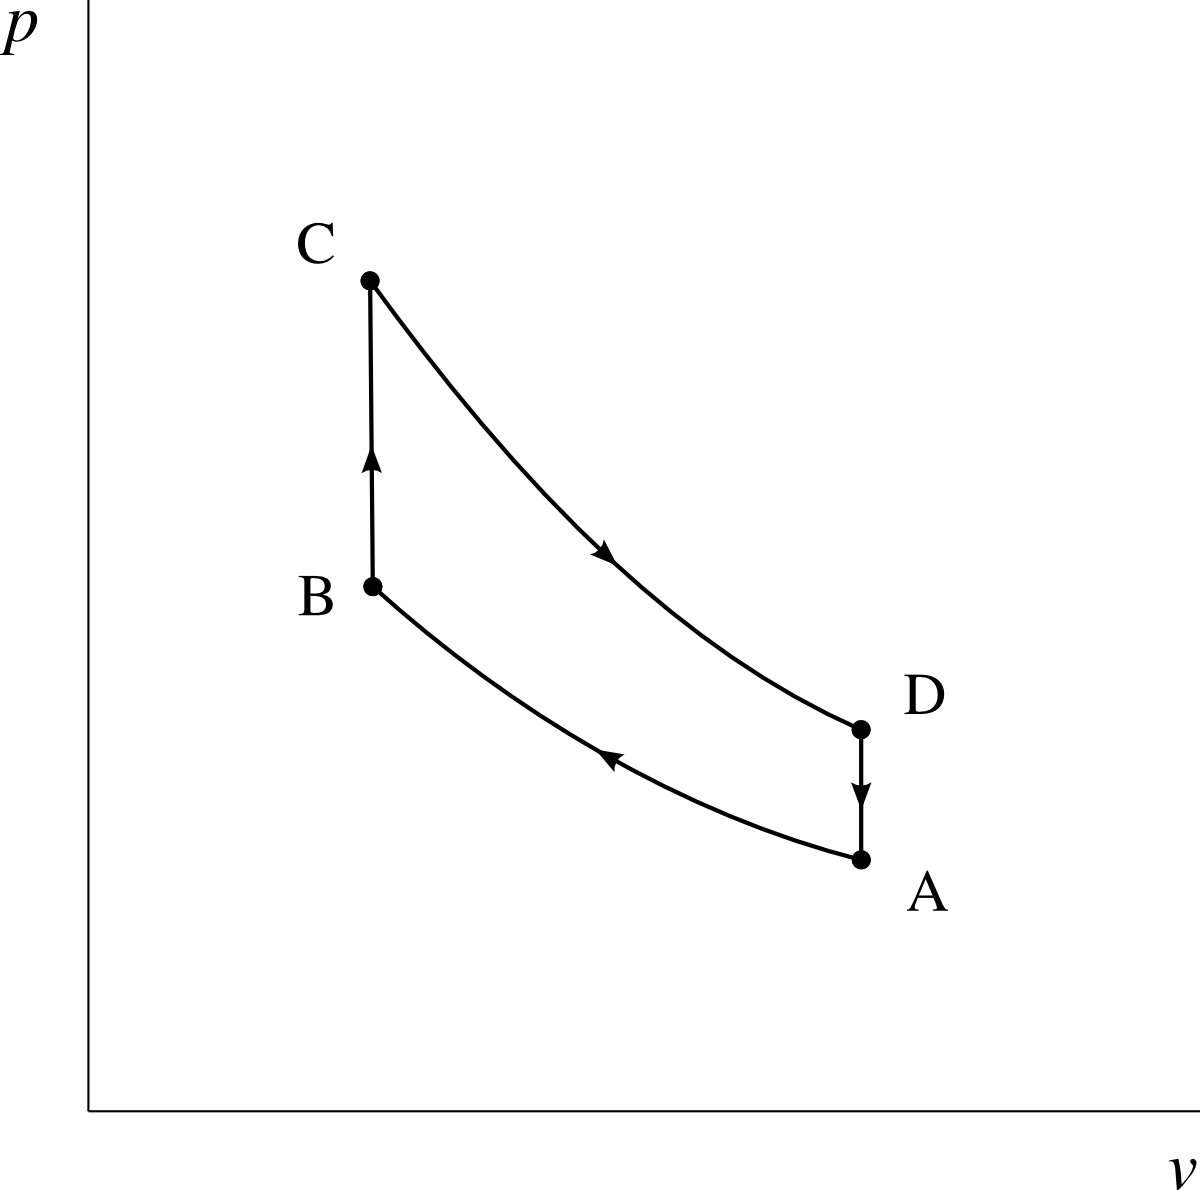
\includegraphics[width=0.45\textwidth]{images/pv_gp_otto.png}
				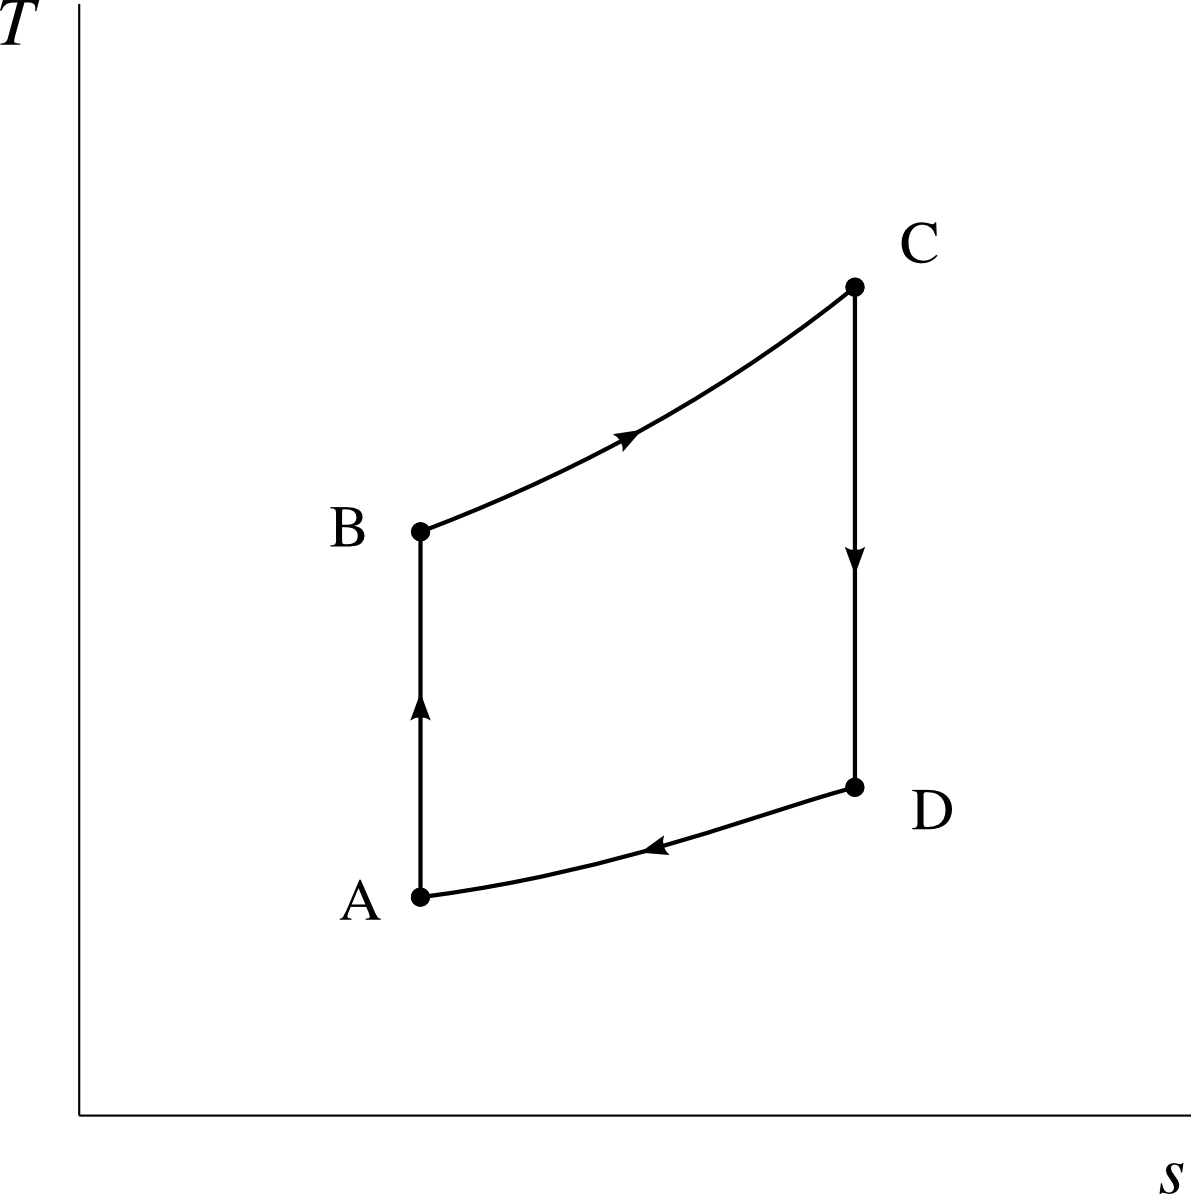
\includegraphics[width=0.45\textwidth]{images/ts_gp_otto.png}
			\end{center}
			\supercaption{Cycle théorique d’Otto représenté sur des diagrammes pression-volume et température-entropie. Ces graphiques représentent le trajet idéal, sans irréversibilité de compression ou détente.}{diagrammes \cczero \oc}
			\label{fig_cycle_otto}
		\end{figure}

		Le cycle d’Otto est conçu pour permettre une mise en œuvre simple de la phase d’apport de chaleur. Le carburant est mélangé à l’air avant son insertion dans le moteur, et une combustion très rapide est provoquée avec une étincelle lorsque le volume dans le cylindre est minimal : c’est ce que l’on nomme l’\vocab{allumage commandé}. Otto destine son moteur à des applications statiques, mais sa simplicité relative et sa réactivité assureront son succès dans les transports (notamment avec son fils \wf{Gustav Otto}, avionneur dont l’entreprise donnera naissance à \textsc{bmw}).

		Le rendement du cycle d’Otto théorique est calculable sans grande difficulté. L’apport de chaleur $q_\text{combustion} = c_v (T_\C - T_\B )$ et le rejet de chaleur $q_\text{refroidissement} = c_v (T_\A - T_\D)$ sont tous deux effectués à volume constant\footnote{Le refroidissement, en pratique, est effectué hors du moteur (à la sortie du pot d’échappement). D’un point de vue thermodynamique, l’air poursuit son cycle dans l’atmosphère avant de pénétrer à nouveau dans le moteur (\S\ref{ch_construction_cycle}).} (\ref{eq_q_gp_sf_isochore}). Ainsi, puisqu’en théorie aucun transfert de chaleur n’a lieu dans les phases de compression et détente, et si l’on considère que les propriétés ($c_v$) du gaz ne changent pas pendant la combustion, le rendement $\eta_\text{Otto}$ du cycle théorique est simplement :
		\begin{equation}
			\eta_\text{Otto} = \left| \frac{-q_\text{combustion} - q_\text{refroidissement}}{q_\text{combustion}} \right| = 1 + \frac{q_\text{refroidissement}}{q_\text{combustion}} = 1 + \left( \frac{T_\A - T_\D}{T_\C - T_\B } \right) \label{eq_tmp_rendement_otto}
		\end{equation}

		En définissant le \vocab{taux de compression} $r_v$ comme :
		\begin{equation}
			r_v \equiv  \frac{v_\A}{v_\B}
		\end{equation}
		il est possible de montrer que l’\cref{eq_tmp_rendement_otto} peut être reformulée pour exprimer le rendement selon :
		\begin{equation}
			\eta_\text{Otto} = 1 - \frac{1}{r_v^{\gamma -1}}
		\end{equation}

		On constate ainsi que le rendement du moteur d’Otto dépend uniquement du taux de compression --\ et non de la quantité de chaleur apportée pendant la combustion\footnote{L’étudiant/e n’aura pas tort de se surprendre de ce résultat --\ la température maximale du cycle n’a pas d’influence sur le rendement ! Dans ce cycle, l’augmentation de la température moyenne d’apport de chaleur est exactement compensée par l’augmentation de la température moyenne de refroidissement.}. Cette équation n’est valide qu’en négligeant le changement des propriétés de l’air pendant la combustion, ainsi que les irréversibilités lors de la compression et de la détente. Il ne faut donc l’utiliser qu’avec la plus grande prudence ; toutefois la tendance qu’elle décrit reste valide, et les motoristes cherchent continuellement à augmenter le taux de compression de leurs moteurs pour en augmenter l’efficacité. Une limite immédiate à ce taux est la température à laquelle le mélange air-carburant s’enflamme spontanément, provoquant une combustion prématurée.

	\subsection{Le cycle de Diesel}
	\label{ch_cycle_diesel}

		\thermoquotebegin{O}
			[Nous souhaitons] produire la température la plus haute du cycle (la température de combustion) non pas par et pendant la combustion, mais avant et indépendament d’elle, entièrement par la compression d’air ordinaire. […]
Le combustible, ainsi, ne doit pas être précédemment mélangé à l’air, mais ce dernier doit être comprimé séparément, sinon, bien avant que la compression requise ne soit atteinte, l’allumage se produirait, et le cycle serait interrompu.
		\thermoquoteend{Rudolf Diesel, 1893~\cite{diesel1893, diesel1893en}}{}
		
		Fruit du travail patient et soigneux de son inventeur, l’ingénieur allemand \wf{Rudolf Diesel}, le \vocab{moteur Diesel} propulse aujourd’hui l’écrasante majorité des transports commerciaux sur route et sur mer.

		D’un point de vue strictement thermodynamique, le cycle de Diesel théorique ne diffère de celui d’Otto que par son mode de combustion : l’apport de chaleur se fait à pression constante et non à volume constant, comme montré en \cref{fig_cycle_diesel}.

		\begin{figure}
			\begin{center}
				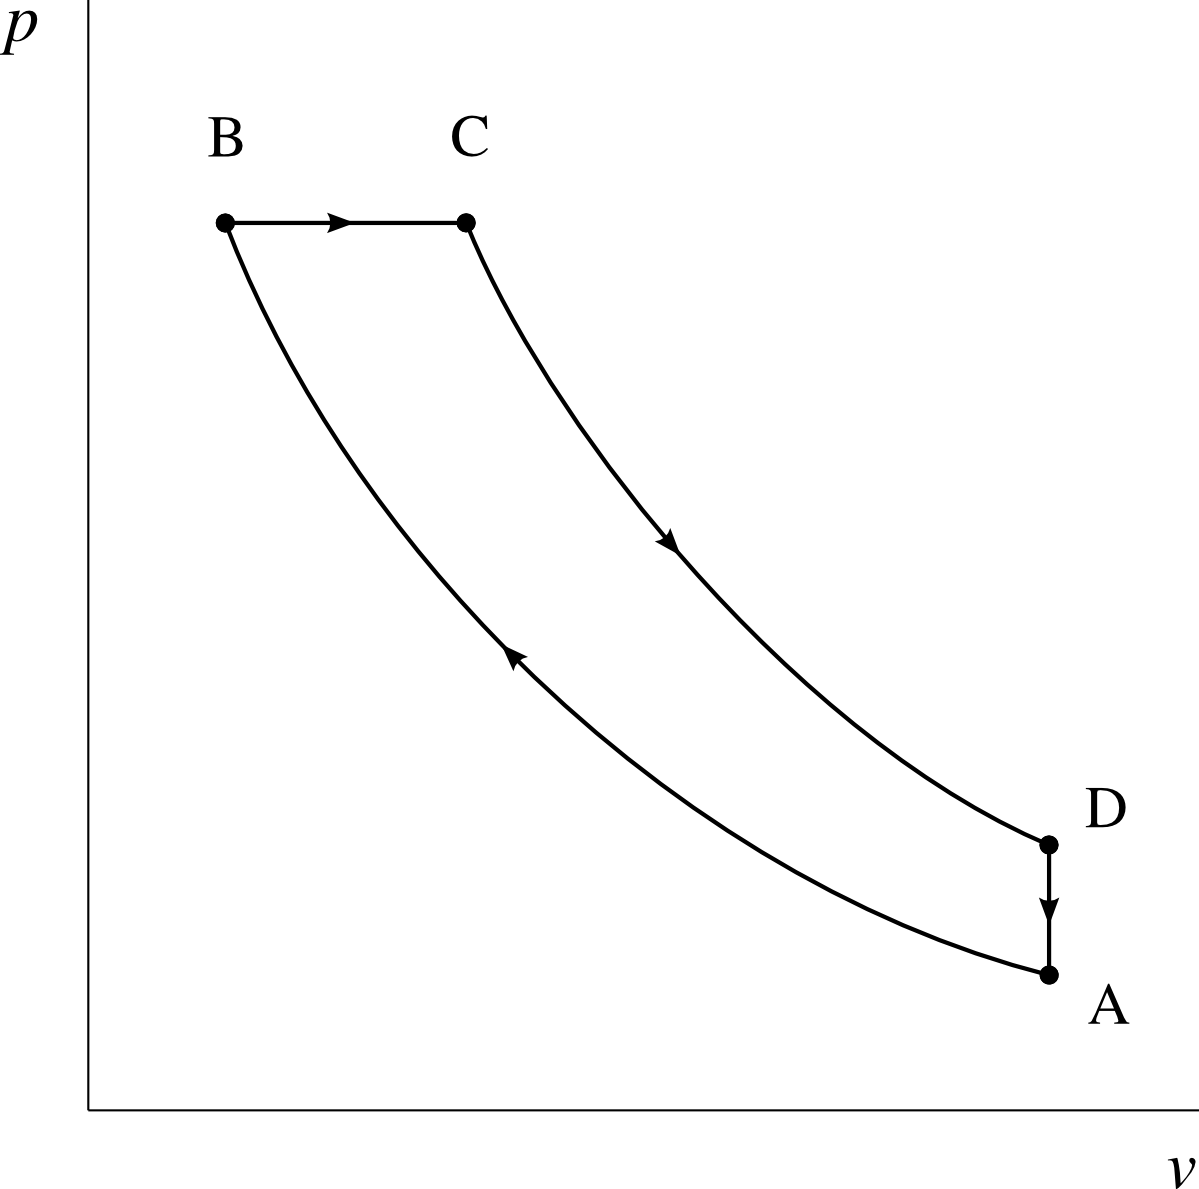
\includegraphics[width=0.45\textwidth]{images/pv_gp_diesel.png}
				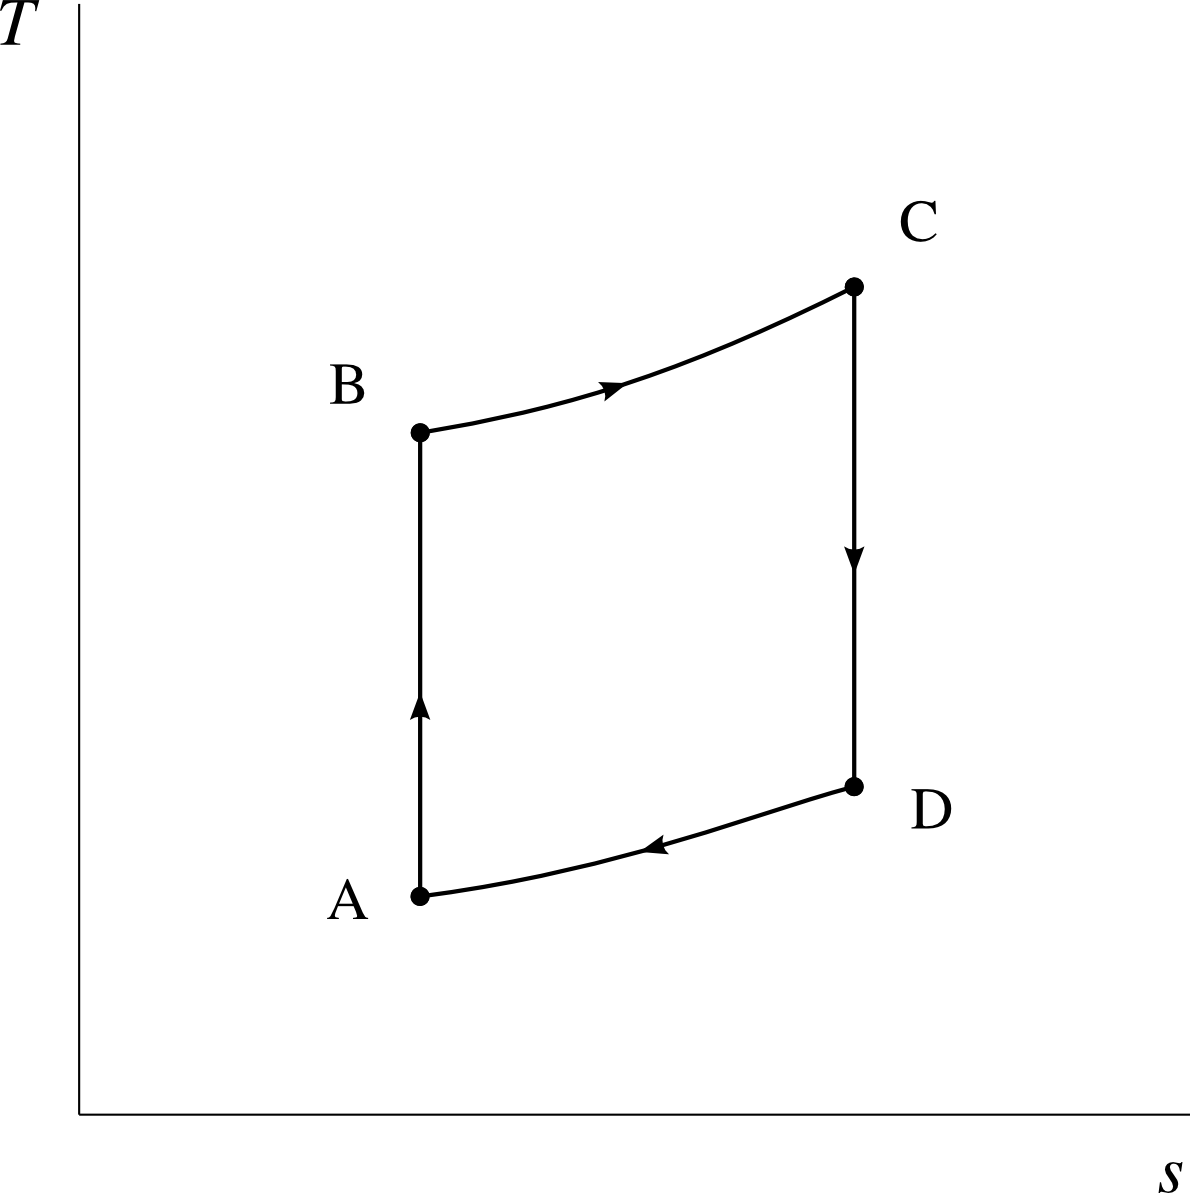
\includegraphics[width=0.45\textwidth]{images/ts_gp_diesel.png}
			\end{center}
			\supercaption{Cycle théorique de Diesel représenté sur des diagrammes pression-volume et température-entropie.	Ces graphiques représentent le trajet idéal, sans irréversibilité de compression ou détente.}{diagrammes \cczero \oc}
			\label{fig_cycle_diesel}
		\end{figure}

		Comme l’apport de chaleur $q_\text{combustion} = c_p (T_\C - T_\B)$ (\ref{eq_q_gp_sf_isobare}) est fait conjointement à une production de travail, il n’existe pas d’expression simple pour le rendement $\eta_\text{Diesel}$, qui ne dépend plus uniquement du taux de compression. Il faudra le calculer en étudiant le cycle étape par étape. On s’apercevra alors que toutes choses étant égales par ailleurs (même taux de compression et même température maximale), le cycle de Diesel a un rendement plus faible que celui d’Otto. 
		
		Pour comprendre, alors, l’intérêt de ce cycle et la différence véritable entre un moteur Diesel et un moteur essence, il faut un peu de contexte historique. Rudolf Diesel conçoit en 1892 un moteur «~rationnel~» pour mettre en pratique le cycle de Carnot. Il recherche donc deux caractéristiques :
		\begin{itemize}
			\item un fort taux de compression, pour augmenter la température de l’air avant la combustion ;
			\item une combustion à température constante.
		\end{itemize}
		Pour obtenir cela, il lui faut attendre la fin de la compression pour injecter le carburant, afin d’éviter un allumage prématuré. L’apport de chaleur isotherme demande quant à lui une combustion progressive. Ainsi, le moteur Diesel originel est par nature doté d’une \vocab{injection directe} de carburant, indépendante de l’admission d’air. Le cycle de Diesel est donc intéressant car il \emph{permet} un taux de compression et une qualité de combustion supérieurs à ceux du cycle d’Otto.
		
		Le moteur de Diesel ne cessera d’évoluer depuis l’impraticable concept décrit dans la \textit{Théorie et construction d’un moteur rationnel à chaleur destiné à remplacer les machines à vapeur et moteurs à combustion connus à ce jour} de 1893~\cite{diesel1893,diesel1893en} (\SI{400}{\bar} et combustion isotherme de poudre de charbon) jusqu’aux premiers modèles de série qu’il développe chez le motoriste \textsc{man} (\SI{40}{\bar} et combustion isobare de pétrole). Tout comme Otto, Diesel s’intéresse d’abord aux moteurs stationnaires (ses premiers prototypes sont monocylindres et dépassent trois mètres de haut) mais ce sont les applications aux transports commerciaux, où l’absence de bougie et son excellent rendement lui donnent l’avantage sur les moteurs à allumage commandé, qui feront sa notoriété. 

	\subsection{Mise en pratique des cycles}
	\label{ch_cycles_pistons_reels}

		Les deux cycles décrits plus haut ne sont que des cycles idéaux --\ ils servent d’étalons conceptuels pour comparer les moteurs réels entre eux. Leur transposition à un moteur réel nécessite de prendre en compte de nombreux facteurs, parmi lesquels :
		\begin{itemize}
			\item La nécessité de vidanger l’air et les produits de combustion à l’intérieur du cylindre après le cycle, et l’impossibilité de le faire complètement ;
			\item Le fait que le volume occupable par le gaz soit lié à la rotation de l’arbre du moteur, et donc qu’il n’est pas possible de le contrôler indépendamment du régime de fonctionnement du moteur ;
			\item Les irréversibilités lors des compressions et détentes causées par les mouvements rapides des pistons ;
			\item Les transferts de chaleur vers et depuis les cylindres pendant le cycle ;
			\item Les fuites des gaz dans les interstices entre pistons et cylindres.
		\end{itemize}

		La prise en compte de ces facteurs, ainsi que la poursuite d’objectifs liés au confort d’utilisation et à la maîtrise de la pollution atmosphérique, font que le cycle obtenu à l’intérieur d’un cylindre de moteur en pratique pourra par exemple ressembler à celui représenté en \cref{fig_cycle_otto_reel}. Dans le secteur automobile en particulier, l’adoption de l’injection directe et l’augmentation des taux de compression sur les moteurs essence pour diminuer leur consommation et leurs émissions a brouillé la distinction essence/Diesel -- les moteurs essence sont désormais plus proches du concept de Rudolf Diesel que de celui de Nikolaus Otto.

		\begin{figure}
			\begin{center}
				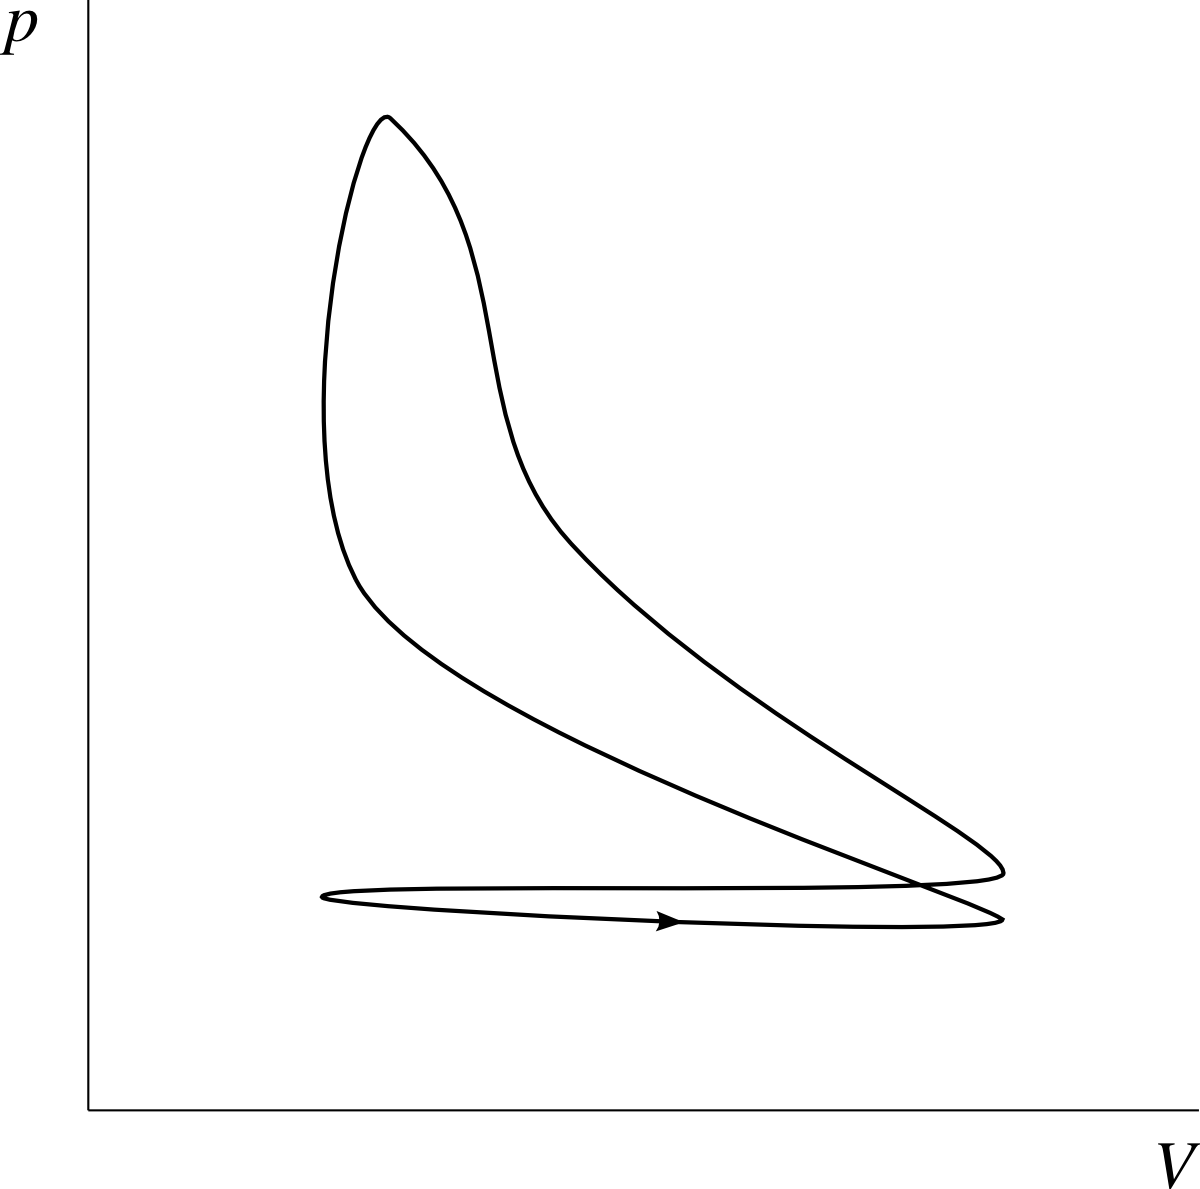
\includegraphics[width=\didacticpvdiagramwidth]{images/pv_moteur_reel.png}
			\end{center}
			\supercaption{Une représentation réaliste de l’évolution de la pression et du volume pendant un cycle dans un moteur essence en pratique.}{diagramme \cczero \oc}
			\label{fig_cycle_otto_reel}
		\end{figure}


	\subsection{Nombre de cylindres et turbocompression}
	\label{ch_turbo}

		Un défaut important des moteurs à mouvement alternatif est que l’irréversibilité des compressions et détentes augmente fortement avec la vitesse d’évolution des pistons dans les cylindres. L’approche traditionnelle pour contourner ce problème est de multiplier le nombre de cylindres fonctionnant simultanément dans le moteur (\cref{fig_beaucoup_cylindres}). De cette façon, on peut réduire le débattement parcouru par chaque piston pour un volume de cylindrée donné. Un avantage associé à cette approche est que le mouvement des pièces mécaniques est mieux équilibré (et le moteur plus mélodieux !).
		
		\begin{figure}
			\begin{center}
				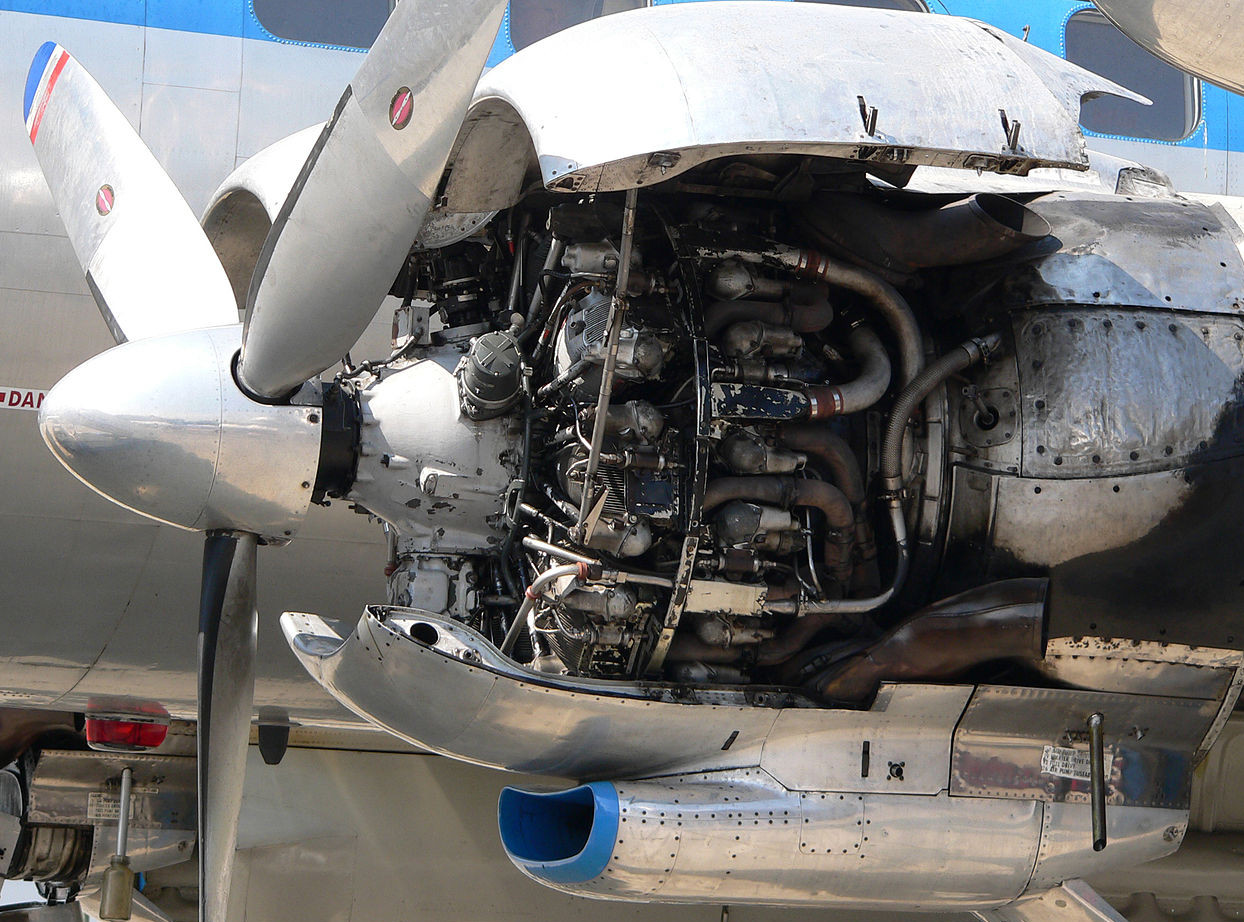
\includegraphics[height=0.325\textwidth]{images/curtiss_wright_cyclone.jpg}
				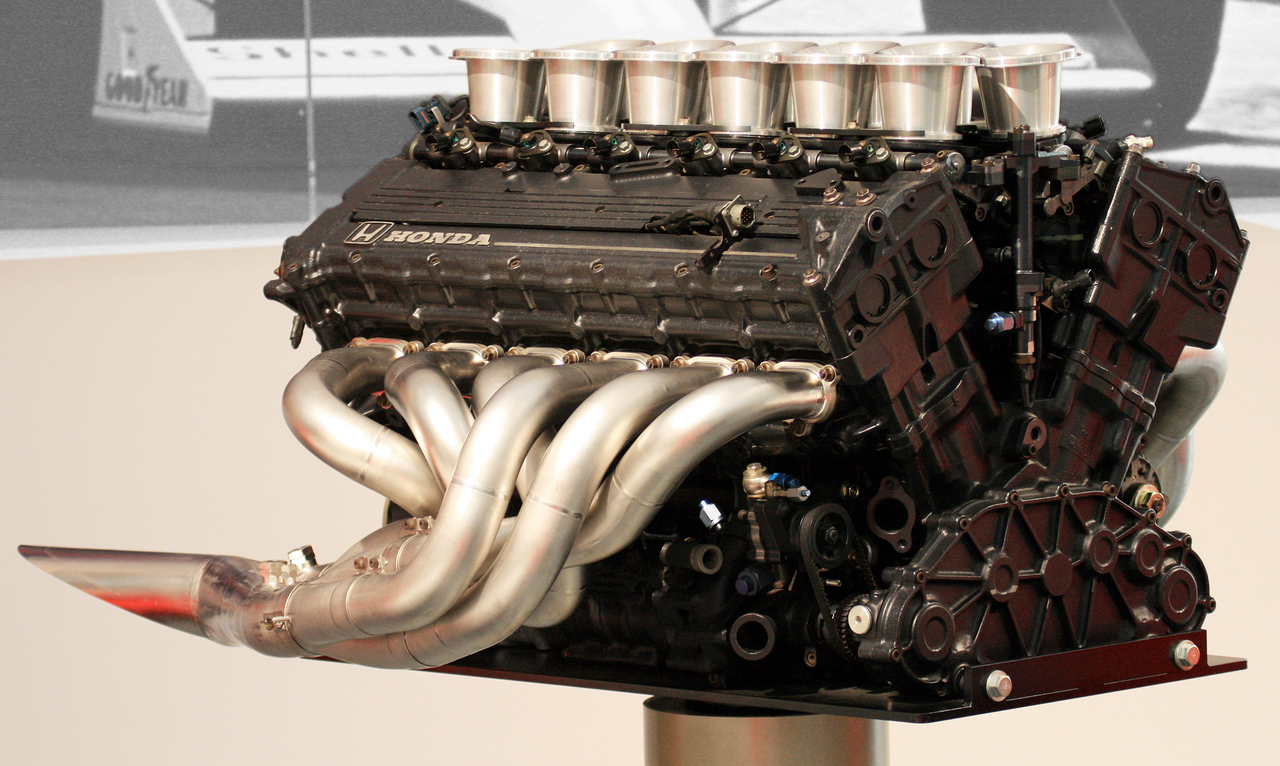
\includegraphics[height=0.325\textwidth]{images/honda_v12.jpg}
			\end{center}
			\supercaption{À gauche, un \textit{Curtiss-Wright} \textsc{r-3350} \textit{Duplex-Cyclone} (1950) de \SI{3500}{ch} à 18 cylindres disposés en deux étoiles successives. Quatre de ces moteurs équipaient le long-courrier \textit{Lockheed Super Constellation}.\\
			À droite, un \textit{Honda} \textsc{ra121e} (1991) de 12 cylindres. Il équipait la Formule 1 \textit{McLaren} \textsc{mp4/6}.}{\wcfile{Curtiss Wright Cyclone 1 fcm.jpg}{photo du Duplex-Cyclone} \ccbysa par \wcun{Frank C. Müller}{Frank C. Müller}\\
 \wcfile{Honda RA121E engine front Honda Collection Hall.jpg}{photo du V12 \textsc{ra121e}} \ccbysa par \wcu{Morio}}
			\label{fig_beaucoup_cylindres}
		\end{figure}
		
		Malheureusement, la complexité mécanique, l’encombrement et les coûts de fabrication et d’entretien des moteurs augmentent rapidement avec le nombre de cylindres ; ainsi dans les applications où ces facteurs priment (pour la majorité du secteur automobile, par exemple) on n’utilise généralement que quatre, voire trois cylindres. Il est pourtant attendu de ces moteurs qu’ils puissent être efficaces sur une large plage de puissances.
	
		Une solution couramment adoptée pour cela est celle de la \vocab{turbocompression}. Elle consiste à déléguer une partie du travail de compression et de détente à un petit appareil nommé \vocab{turbo}, qui apporte avec lui les avantages de compacité et de légèreté des turbomachines (\cref{fig_turbo}). Le compresseur du turbo est alimenté par sa turbine, qui fonctionne avec les gaz d’échappement (nous étudions ce système plus bas en~\S\ref{ch_generateur_gaz}). La turbocompression permet de réduire la taille et la vitesse d’un moteur pour une puissance donnée.
		
		\begin{figure}
			\begin{center}
				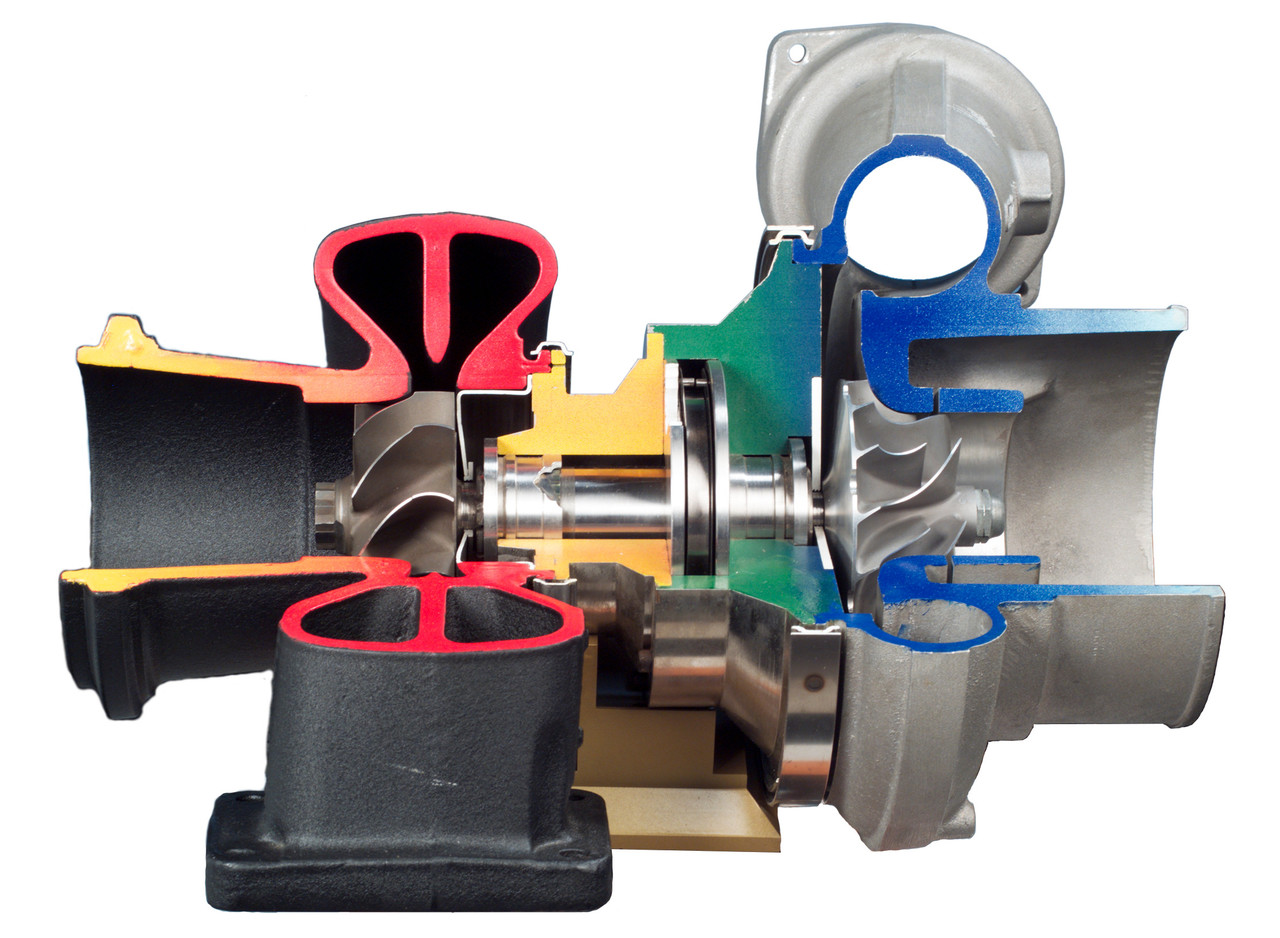
\includegraphics[width=0.6\textwidth]{images/coupe_turbo.jpg}
			\end{center}
			\supercaption{Un turbo sectionné pour en montrer l’agencement intérieur. L’air atmosphérique entre par la droite et est comprimé en étant projeté vers l’extérieur par le compresseur centrifuge ; il est ensuite inséré dans le moteur. Les gaz d’échappement pénètrent par le centre gauche et ressortent vers la gauche après avoir fait tourner la turbine centripète, qui alimente le compresseur en travail \textit{via} l’arbre central de rotation. Comme l’unique pièce mobile est très compacte (ici environ~\SI{20}{\centi\metre}), de très grandes vitesses de rotation peuvent être atteintes, usuellement au delà de~\SI{200 000}{tours/min}.}{\wcfile{Turbocharger.jpg}{Photo} \pd \textsc{Nasa}}
			\label{fig_turbo}
		\end{figure}
		
		Comme l’utilisation d’un turbo affecte négativement la réactivité d’un moteur, on peut permettre à l’air d’admission de le contourner pendant les variations de régime. De plus, les variations de température dans le turbo peuvent être compensées par refroidissement avant insertion dans les cylindres (nous étudions cette technique plus bas en~\S\ref{ch_intercooling}). Ces procédés font des moteurs modernes des systèmes thermodynamiques complexes capables d’effectuer une large gamme de cycles très différents en fonction des conditions d’utilisation.

\onlyframabook{\clearpage}%handmade ici saut de page, sinon la citation de Carnot casse tout
\section{Composants des turbomachines}

	Avant de nous plonger dans les cycles des moteurs à turbines, nous nous proposons de rappeler brièvement le fonctionnement de leurs principaux composants. Comme les turbomachines fonctionnent en régime permanent, nous ferons à partir d’ici systématiquement appel aux notions du \courstrois.

	\subsection{Compresseur}
	
		\thermoquotebegin{O}
			Afin de pouvoir donner à l’air une grande extension de volume, afin de produire par cette extension un grand changement de température, il serait nécessaire de le prendre d’abord sous une pression assez élevée […] Cette opération exigerait un appareil particulier, appareil qui n’existe pas dans les machines à vapeur. Dans celles-ci, l’eau est à l’état liquide lorsqu’on la fait pénétrer dans la chaudière ; elle n’exige, pour y être introduite, qu’une pompe foulante de petites dimensions.
		\thermoquoteend{Sadi Carnot, 1824\cite{carnot1824}}{~}
	
		Les phases de compression et de détente dans les moteurs se font très souvent de façon adiabatique et toujours de façon irréversible. L’écoulement des fluides au sein du compresseur des moteurs modernes est difficile à modéliser\footnote{On sait de la mécanique des fluides que le gradient de pression au sein d’un compresseur favorise la séparation de la \vocab{couche limite}. Ainsi, on utilise toujours un plus grand nombre d’étages dans un compresseur que dans une turbine de même puissance, où le gradient est favorable.}\nolinebreak ; ce qui en fait un composant lourd, volumineux et dont la géométrie est complexe (figures~\ref{fig_schéma_compresseur1} et~\ref{fig_schéma_compresseur2}).\\
		La plupart des compresseurs sont \vocab{axiaux}, c’est à dire que l’air les traverse parallèlement à l’axe de rotation, mais on utilise parfois des compresseurs \vocab{centrifuges}, qui projettent l’air radialement ; quelque soit le procédé utilisé, les évolutions thermodynamiques de l’air restent identiques.

		\begin{figure}
			\begin{center}
				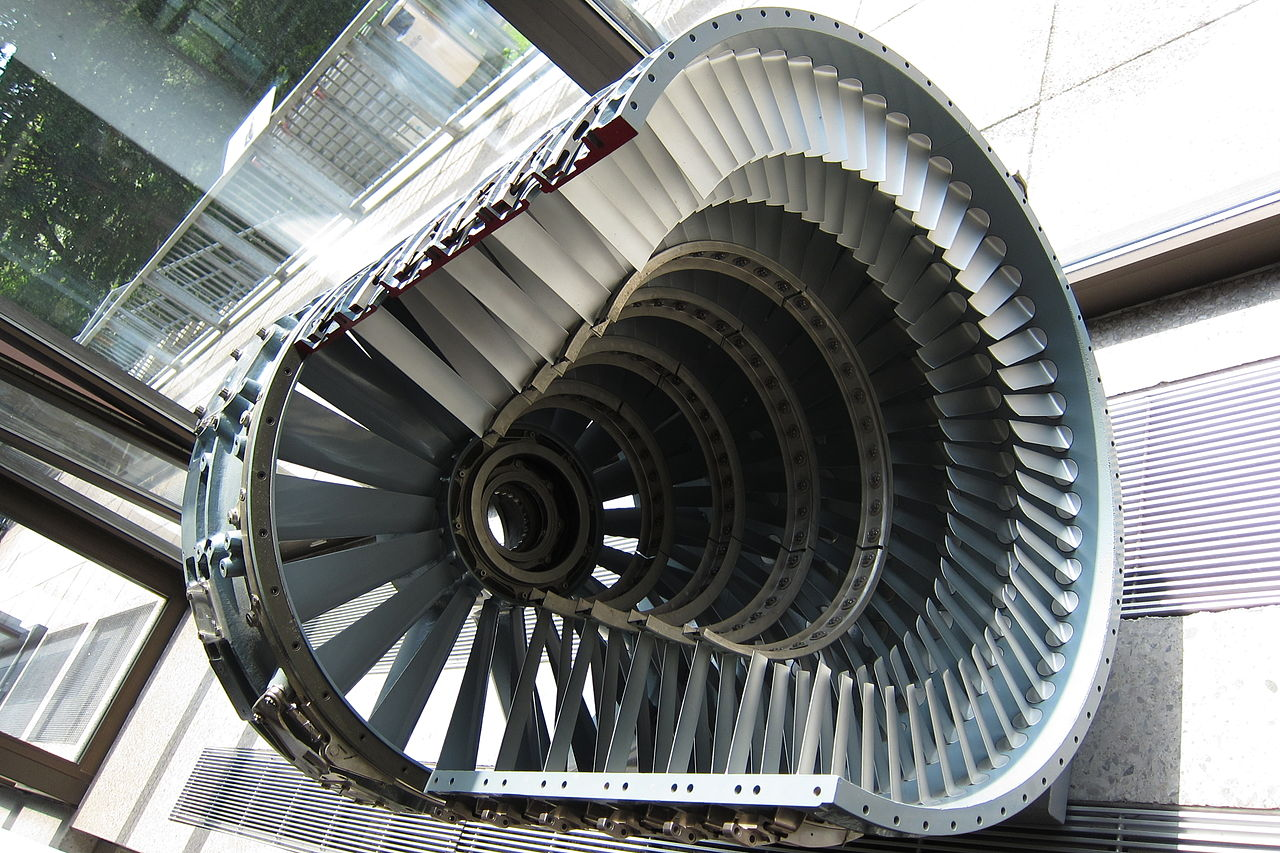
\includegraphics[width=9cm]{images/photo_compresseur.jpg}
			\end{center}
			\supercaption{Caisson de stators accueillant le rotor d’un compresseur axial d’un turboréacteur.}{\wcfile{Compressor_case_from_turbofan.jpg}{Photo} \ccbysa \olivier}
			\label{fig_schéma_compresseur1}
		\end{figure}

		\begin{figure}
			\begin{center}
				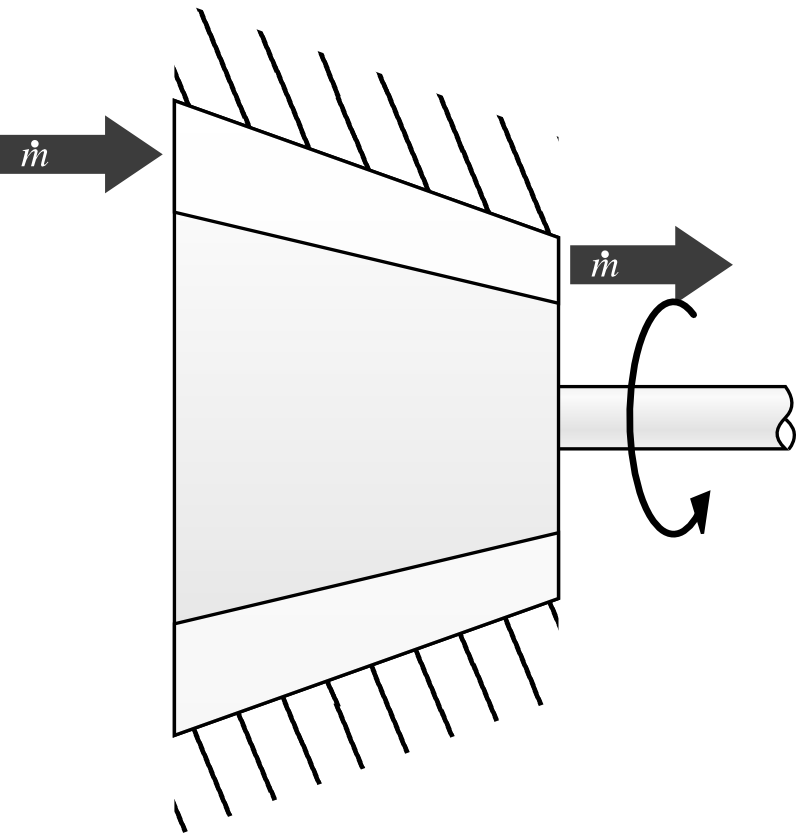
\includegraphics[width=4cm]{images/symbole_compresseur.png}
			\end{center}
			\supercaption{Représentation schématique d’un compresseur à air.}{schéma \ccbysa \olivier}
			\label{fig_schéma_compresseur2}
		\end{figure}

		Tout comme nous l’avons fait pour la turbine (\ref{def_efficacité_isentropique_turbine}), nous quantifions l’efficacité d’un compresseur en comparant sa puissance avec celle d’un compresseur idéal (un compresseur qui serait isentropique). Nous nommons ce paramètre l’\vocab{efficacité isentropique} du compresseur $\eta_\C$ :
		\begin{equation}
			\eta_\C \equiv  \frac{\dot W_\text{compresseur isentropique}}{\dot W_\text{compresseur réel}}
			\label{def_efficacité_isentropique_compresseur}
		\end{equation}
		\begin{equationterms}
			\item pour un compresseur ;
			\item où \tab $\dot W_\text{compresseur réel}$ \tab\tab\tab est la puissance réelle consommée par le compresseur,
			\item et \tab $\dot W_\text{compresseur isentropique}$ \tab la puissance d’un compresseur isentropique qui fonctionnerait avec le même débit de masse et entre les deux mêmes pressions.
		\end{equationterms}

		Comme celle d’une turbine, l’efficacité isentropique d’un compresseur est toujours inférieure à~1. Si cette efficacité est connue, nous pouvons comparer les propriétés réelles de l’air à l’entrée et à la sortie du compresseur avec celles que l’on mesurerait dans le cas idéal :
		\begin{equation}
			w_\text{compresseur} = c_p \ (T_\text{B réel} - T_\A) = \frac{1}{\eta_\C} c_p \ (T_{\B’} - T_\A)
			\label{eq_puissance_compresseur}
		\end{equation}
		\begin{equationterms}
			\item où \tab $w_\text{compresseur}$ 	\tab est la puissance spécifique du compresseur (\si{\joule\per\kilogram}),
			\item 	\tab $T_{\B’}$ 					\tab\tab\tab est la température idéale de sortie (compresseur isentropique) (\si{\kelvin}),
			\item et \tab $T_\text{B réel}$ 			\tab est la température réelle de sortie (\si{\kelvin}).
		\end{equationterms}

		\begin{anexample}
			Pour l’air, on mesure $c_{p\text{(air)}} = \SI{1005}{\joule\per\kilogram\per\kelvin}$, $c_{v\text{(air)}} = \SI{718}{\joule\per\kilogram\per\kelvin}$, $R_\text{air} = \SI{287}{\joule\per\kilogram\per\kelvin}$, et $\gamma_\text{air} = \num{1,4}$.\\
			Le compresseur d’un turboréacteur à soufflante a une efficacité isentropique de \SI{85}{\percent} ; il admet \SI{38}{\kilogram\per\second} d’air à \SI{1}{\bar} et \SI{5}{\degreeCelsius}. La pression de sortie est de \SI{40}{\bar}. Quelle est la puissance consommée ?
				\begin{answer}
					L’évolution peut être représentée de façon qualitative sur un diagramme $T-s$ ainsi :
						\begin{center}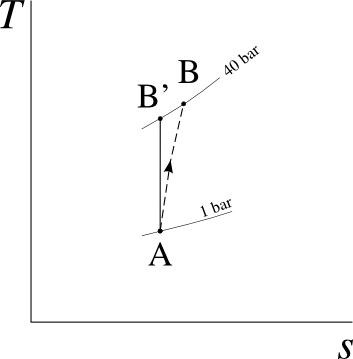
\includegraphics[width=4cm]{images/exe_ts_compresseur.png}\end{center}
					Nous commençons par calculer la puissance d’un compresseur idéal (isentropique) : la température de sortie serait alors (\ref{eq_isentropique_horrible2}) :
						$T_{\B’} = T_\A \left(\frac{p_\B}{p_\A}\right)^{\frac{\gamma - 1}{\gamma}}
					 			= (5 + \num{273,15}) \left(40\right)^{\frac{\num{0,4}}{\num{1,4}}}
					 			= \SI{798}{\kelvin} = \SI{524,9}{\degreeCelsius}$.
					 Le compresseur idéal consommerait donc $w_\text{compresseur isentropique} = c_{p \text{(air)}} \ (T_{\B’} - T_\A) = \num{1005} \ (\num{798} - \num{278,15}) = \SI{+5,225e5}{\joule\per\kilogram} = \SI{+522,5}{\kilo\joule\per\kilogram}$.
					 
					 Avec l’\cref{def_efficacité_isentropique_compresseur} la puissance du compresseur vient naturellement : $\dot W_\text{compresseur} = \dot m \ \frac{1}{\eta_\text{C}} \ w_\text{compresseur isentropique} = \num{38} \times \frac{1}{\num{0,85}} \times \num{5,225e5} = \SI{2,336e7}{\watt} = \SI{23,36}{\mega\watt}$.
					 	\begin{remark}
					 		Attention : contrairement aux turbines, la puissance réelle est \emph{supérieure} à la puissance théorique : on divise par l’efficacité dans le dernier calcul.
					 	\end{remark}
					 	\begin{remark}
					 		L’\cref{eq_puissance_compresseur} nous permettrait de calculer la température réelle de sortie : $T_\text{B réel} = \frac{1}{\eta_\C} c_p \ (T_{\B’} - T_\A) + T_\A = \frac{1}{\num{0,85}} (\num{798} - \num{278,15}) + \num{278,15} = \SI{889,7}{\kelvin} = \SI{616,6}{\degreeCelsius}$. Ici, les \SI{92}{\degreeCelsius} de différence avec le cas isentropique sont le résultat de la conversion de travail en chaleur par frottement dans le compresseur, une dépense inutile représentant $\dot m \ c_p \ (T_\B - T_{\B’}) = \SI{+3,5}{\mega\watt}$.
					 	\end{remark}
				\end{answer}
		\end{anexample}


		En pratique, plusieurs prélèvements d’air peuvent être effectués au sein du compresseur, pour alimenter d’autres équipements et pour refroidir la turbine (\ref{ch_refroidissement_turbine}). Pendant les phases de transition de régime, on peut également soulager le compresseur d’une partie du débit de masse en laissant fuir de l’air au travers de soupapes de décharge.


	\subsection{Chambre de combustion}

		L’apport de chaleur des turbomachines se fait dans une ou plusieurs chambres de combustion (figures~\ref{fig_chambre_de_combustion1} et~\ref{fig_chambre_de_combustion2}). L’air y est réchauffé à pression constante par combustion ; sa température et son volume spécifique augmentent fortement.

		\begin{figure}
			\begin{center}
				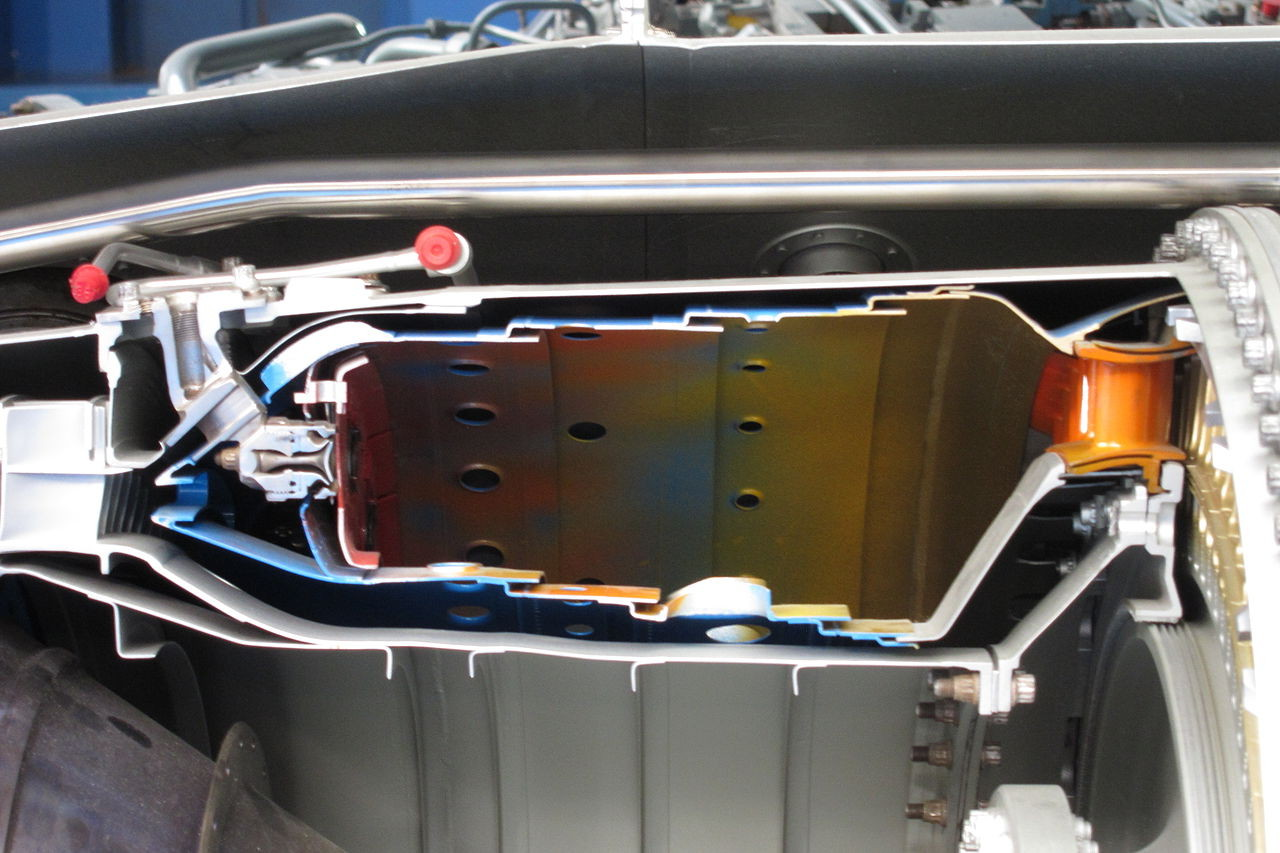
\includegraphics[width=9cm]{images/photo_chambre_combustion.jpg}
			\end{center}
			\supercaption{Section d’une chambre de combustion annulaire dans laquelle l’écoulement se faisait de gauche à droite. La photo montre une découpe d’un \textit{Rolls-Royce Turbomeca Adour}, petit turboréacteur conçu en 1968.}{\wcfile{Combustor_of_sectioned_Rolls-Royce_Turboméca_Adour_turbofan.jpg}{Photo} \ccbysa \olivier}
			\label{fig_chambre_de_combustion1}
		\end{figure}

		\begin{figure}
			\begin{center}
				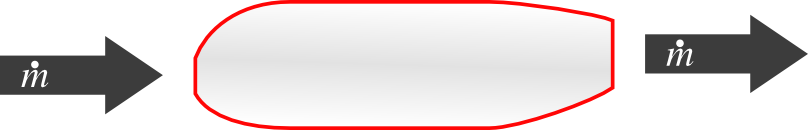
\includegraphics[width=7cm]{images/symbole_chambre_combustion.png}
			\end{center}
			\supercaption{Représentation schématique d’une chambre de combustion.}{schéma \cczero \oc}
			\label{fig_chambre_de_combustion2}
		\end{figure}

		Aucun travail n’est apporté dans la chambre de combustion, et la pression y reste approximativement constante.	Comme l’apport de chaleur se fait au sein du gaz même, la température maximale du cycle n’est pas limitée par la transmission de chaleur à travers une paroi solide. La température maximale de l’air peut même dépasser celle de fonte des parois la chambre, qui sont isolées avec plusieurs couches d’air comprimé. Cela permet un gain de température par rapport aux installations à vapeur qui avoisine usuellement \SI{200}{\kelvin}.

		La puissance délivrée dans la chambre de combustion se quantifie plutôt facilement avec une modification de l’\cref{eq_q_gp_so_isobare} pour tenir compte du changement des propriétés de l’air pendant la combustion, qui fait augmenter la valeur de $c_p$ de~\SI{10}{\percent} environ :
		\begin{equation}
			q_\text{chambre} = h_\B - h_\A = c_{p \text{(gaz)}} T_\B \ - \ c_{p \text{(air)}} T_\A
		\end{equation}

		Les écoulements au sein de la chambre de combustion dépendent de façon corrélée de la chimie de combustion et de la distribution spatiale des vitesses et de la pression : leur modélisation est donc complexe. En pratique une légère perte de pression des gaz est obtenue entre les extrémités des chambres. L’influence sur la puissance du débit massique du carburant $\dot m_\text{carburant}$, toujours beaucoup plus faible que celui de l’air, peut être négligée sans danger.


	\subsection{Turbine}

		Le rôle de la turbine (figures~\ref{fig_illustration_turbine1} et~\ref{fig_illustration_turbine2}) est d’alimenter le compresseur : elle doit donc extraire de l’air une puissance suffisante pour faire fonctionner ce dernier et compenser d’éventuelles pertes de transmission. En fonction de la configuration de la turbomachine, la turbine pourra ensuite extraire encore de l’énergie, pour alimenter d’autres composants, comme nous l’étudions en \S\ref{ch_configurations_turbomachines} plus bas.

		\begin{figure}
			\begin{center}
				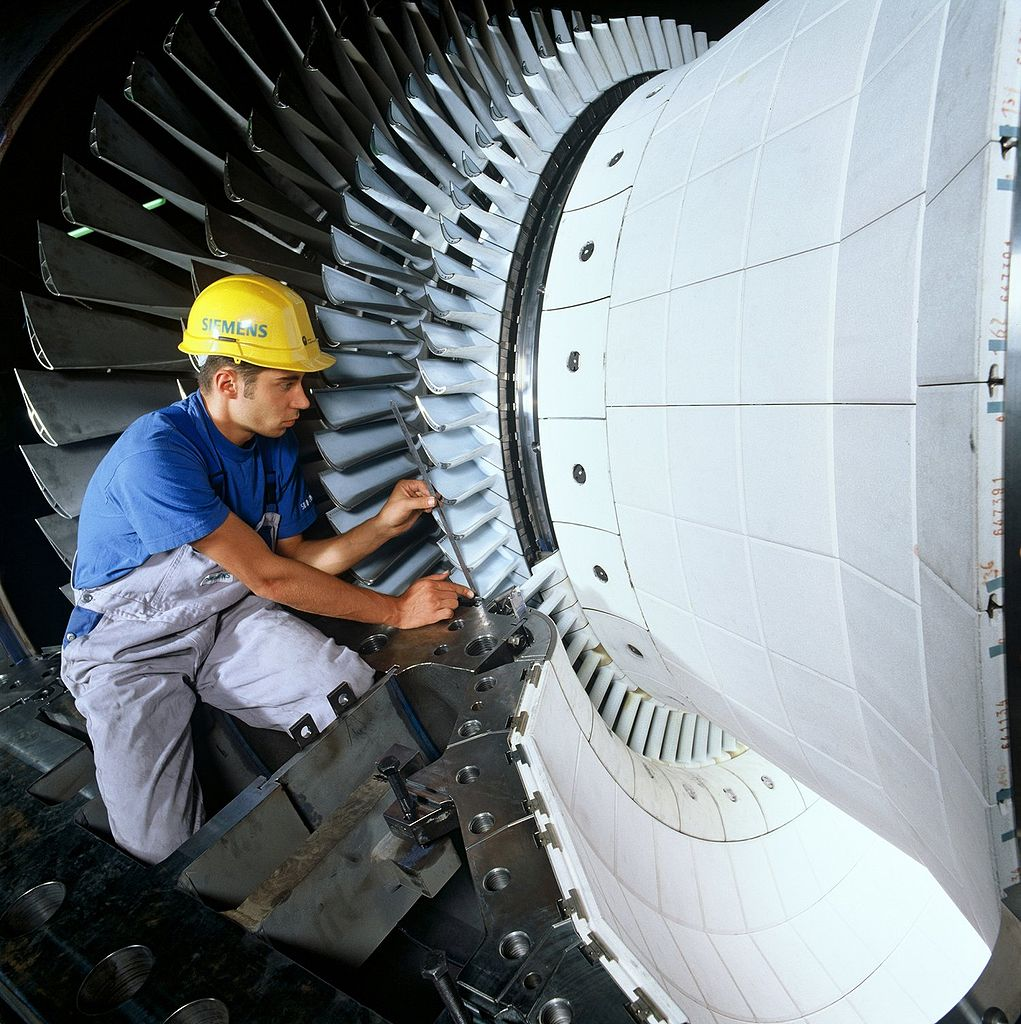
\includegraphics[width=9cm]{images/photo_turbine.jpg}%\hspace{0.2cm}
			\end{center}
			\supercaption{Turbine d’un turbomoteur générateur. La turbine photographiée, une \textit{Siemens} \textsc{sgt5}, peut accepter un débit d’air et d’eau de~\SI{690}{\kilogram\per\second}. Elle transmet une puissance à l’arbre d’environ \SI{500}{\mega\watt}.}{\wcfile{Gasturbine_Montage01.jpg}{photo} \ccbysa Siemens Pressebild}
			\label{fig_illustration_turbine1}
		\end{figure}

		\begin{figure}
			\begin{center}
				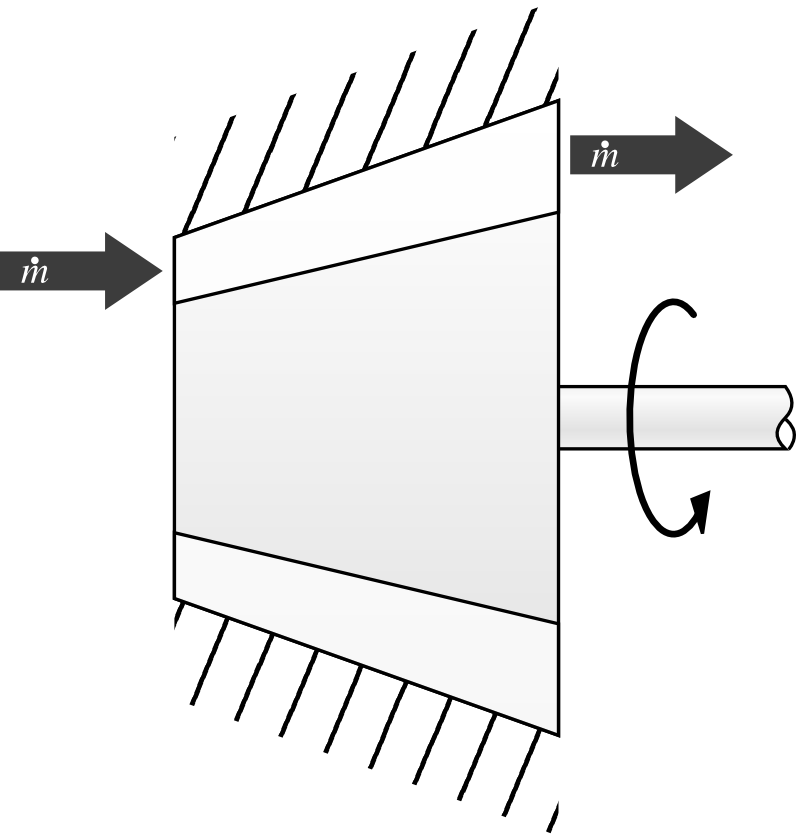
\includegraphics[width=4cm]{images/symbole_turbine.png}
			\end{center}
			\supercaption{Représentation schématique d’une turbine à gaz.}{schéma \ccbysa \olivier}
			\label{fig_illustration_turbine2}
		\end{figure}

		Tout comme pour les liquides/vapeurs (\ref{def_efficacité_isentropique_turbine}), nous mesurons la performance d’une turbine en quantifiant son \vocab{efficacité isentropique} $\eta_\text{T}$ :
		\begin{equation}
			\eta_\text{T} \equiv  \frac{\dot W_\text{Turbine réelle}}{\dot W_\text{Turbine isentropique}}	  \tag{\ref{def_efficacité_isentropique_turbine}}
		\end{equation}

		La puissance extraite par la turbine s’exprime donc aisément en fonction des températures réelle $T_{2~\text{réel}}$ et idéale $T_{2’}$ à sa sortie :
		\begin{equation}
			w_\text{turbine} = c_{p \text{(gaz)}} (T_{2~\text{réel}} - T_1) =  \eta_\text{T} \ c_{p \text{(gaz)}} \ (T_{2’} - T_1)
			\label{eq_puissance_turbine_gaz}
		\end{equation}

		Au fur et à mesure que le gaz circule d’amont en aval de la turbine, il est détendu et son volume spécifique augmente. La taille des pales (donc leur poids et leur coût) doit donc aussi augmenter, tandis que la puissance qu’il leur est possible d’extraire, elle, diminue. Il arrive ainsi souvent que l’on rejette de l’air encore comprimé à la sortie d’une turbomachine, faute de pouvoir en extraire encore de l’énergie de façon économique.


	\subsection{Tuyère}

		\thermoquotebegin{O}
			Lorsqu’en effet deux fluides également comprimés s’échappent par deux petits orifices égaux, leurs vîtesses sont en raison inverse de la racine carrée de leurs \mbox{densités}.% accent sur vîtesses tel quel dans le texte original
		\thermoquoteend{Louis Joseph Gay-Lussac, 1807~\cite{gaylussac1807}}{~}

		La \vocab{tuyère} est un simple conduit sans pièce mobile (figures~\ref{fig_illustration_tuyere1} et~\ref{fig_illustration_tuyere2}). Elle permet au gaz de se détendre, et ainsi d’accélérer vers l’arrière du moteur. C’est cette augmentation de la vitesse du gaz (différence entre vitesse à l’entrée et à la sortie) qui est à l’origine de la poussée fournie par un moteur.

		Il n’y a aucun apport de chaleur ou de travail dans la tuyère : si l’on néglige les frottements, l’énergie du gaz est conservée. La tuyère est le seul élément du moteur pour lequel la variation d’énergie cinétique doit être impérativement prise en compte.

		\begin{figure}
			\begin{center}
				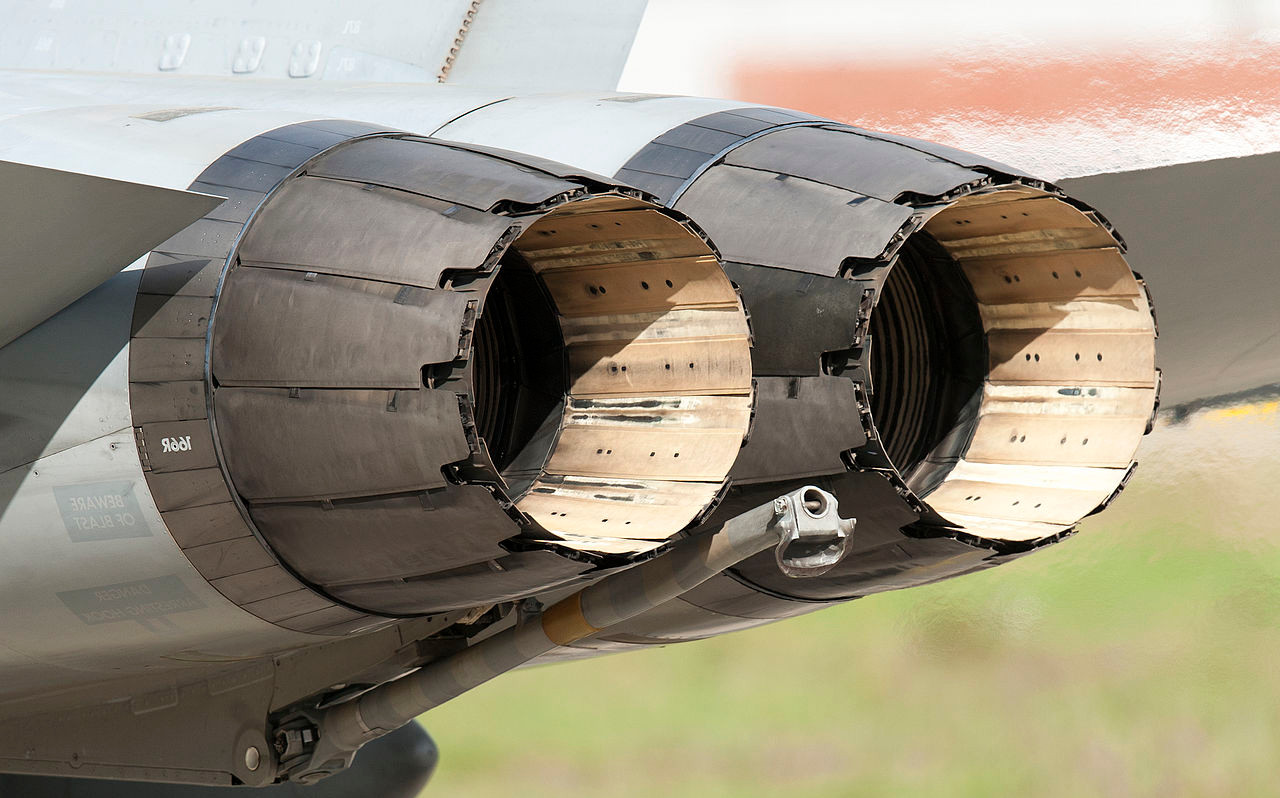
\includegraphics[width=8cm]{images/photo_tuyere.jpg}
			\end{center}
			\supercaption{Les tuyères de deux \textit{General Electric} \textsc{f404} équipant un avion de combat. La géométrie de la tuyère, d’importance capitale en mécanique des fluides, n’est pas abordée dans ce document.}{\wcfile{1280px-Swiss_F-18_Hornet.jpg}{photo} \ccbysa par \href{http ://www.flickr.com/people/39270009@N02}{Peng Chen}}
			\label{fig_illustration_tuyere1}
		\end{figure}

		\begin{figure}
			\begin{center}
				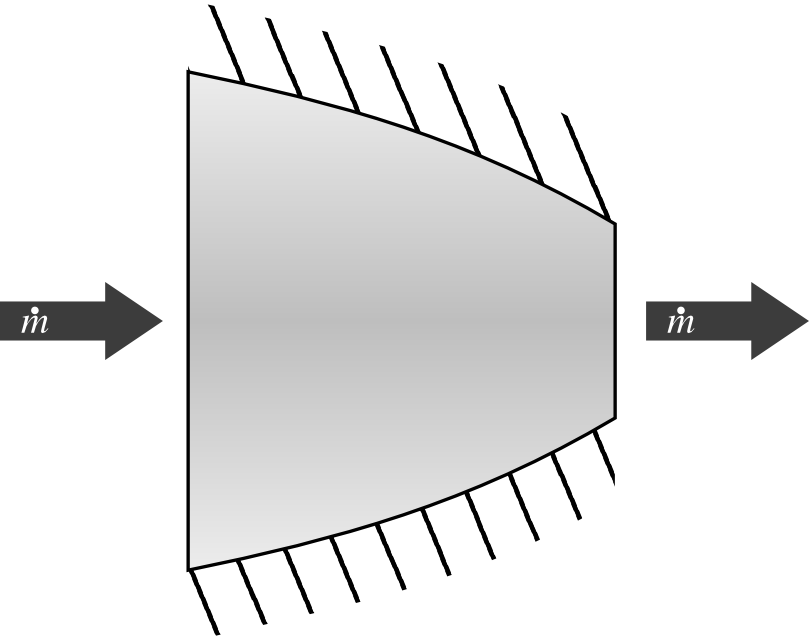
\includegraphics[width=5cm]{images/symbole_tuyere.png}
			\end{center}
			\supercaption{Représentation schématique d’une tuyère.}{schéma \cczero \oc}
			\label{fig_illustration_tuyere2}
		\end{figure}

		Un rapide retour à l’\cref{eq_petite_sfee_deltas_h} nous permet de quantifier la vitesse finale des gaz en fonction de la différence de pression disponible :
		\begin{IEEEeqnarray}{rCl}
			q_{\A \to \B} + w_{\A \to \B} 		& = & \Delta h + \Delta e_{m}  		\ztag{\ref{eq_petite_sfee_deltas_h}}\\
			h_\A + \frac{1}{2} C_\A^2		& = & h_\B + \frac{1}{2} C_\B^2
		\end{IEEEeqnarray}

		Dans le cas d’une tuyère idéale, la détente est isentropique et nous pouvons relier les températures $T_\A$ et $T_\B$ tout comme au sein d’une turbine ou d’un compresseur, par les abominables relations \ref{eq_isentropique_horrible1} à \ref{eq_isentropique_horrible3}. Ainsi, en connaissant les conditions d’entrée $h_\A$ et $p_\A$, pour une pression de sortie $p_\B$ donnée (pression atmosphérique), nous pouvons quantifier la variation de vitesse du gaz :
		\begin{equation}
			C_\B^2 - C_\A^2 	= - 2 \ c_{p \text{(gaz)}} \ (T_\B - T_\A)
			\label{eq_vitesses_tuyere}
		\end{equation}

		Idéalement, la tuyère détend les gaz jusqu’à pression ambiante et convertit toute la variation d’enthalpie des gaz en énergie cinétique. En pratique, bien sûr, une partie de cette énergie est convertie en chaleur par frottement. L’efficacité des tuyères est mesurée de façon similaire à celle des compresseurs et turbines, et n’est pas étudiée dans ce document.

		\begin{anexample}
		\label{exemple_tuyere}
			Pour les gaz brûlés, on mesure $c_{p\text{(gaz)}} = \SI{1150}{\joule\per\kilogram\per\kelvin}$, $c_{v\text{(gaz)}} = \SI{823}{\joule\per\kilogram\per\kelvin}$, $R_\text{gaz} = \SI{327}{\joule\per\kilogram\per\kelvin}$, et $\gamma_\text{gaz} = \num{1,333}$.\\
			Une tuyère admet un débit d’air continu à \SI{2}{\bar}, \SI{10}{\metre\per\second} et \SI{400}{\degreeCelsius}. À quelle vitesse peut-elle accélérer ces gaz en les rejetant à \SI{1}{\bar}, si on néglige les irréversibilités ?
				\begin{answer}
					Le cas permettant la plus grande vitesse d’éjection est le cas d’une détente isentropique, alors 
					$T_\B = T_\A \left(\frac{p_\B}{p_\A}\right)^{\frac{\gamma - 1}{\gamma}}
					 			= (400 + \num{273,15}) \left(\frac{1}{2}\right)^{\frac{\num{0,333}}{\num{1,333}}}
					 			= \SI{566,1}{\kelvin} = \SI{293}{\degreeCelsius}$.
					Une telle évolution peut être représentée de façon qualitative sur un diagramme $T-s$ ainsi :
						\begin{center}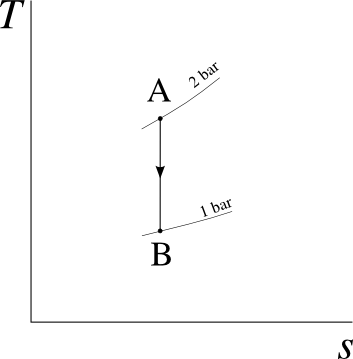
\includegraphics[width=4cm]{images/exe_ts_tuyere.png}\end{center}
					Avec l’\cref{eq_vitesses_tuyere} la vitesse de sortie serait donc 
					$C_\B = \left[ - 2 \ c_{p \text{(gaz)}} \ (T_\B - T_\A) - C_\A^2 \right]^{\frac{1}{2}}
							= \left[ - 2 \times \num{1150} \times (\num{293} - \num{400}) + \num{10}^2 \right]^{\num{0,5}}
							= \SI{496,2}{\metre\per\second} = \SI{1786}{\kilo\metre\per\hour}$.
								\begin{remark}
									Dans la réalité, les gaz n’atteindraient jamais cette vitesse. En effet, une grande partie de la détente se fait \emph{en dehors} de la tuyère, où elle est très turbulente et donc très irréversible.\\
									Ce phénomène, malgré tout, n’a pas d’influence sur la poussée générée par la tuyère, car sa bouche de sortie est en réalité à pression supérieure à la pression atmosphérique. Le calcul de vitesse effectué ici reste ainsi un bon «~indicateur~» thermodynamique des phénomènes en jeu. Pour décrire rigoureusement l’écoulement dans une tuyère, il faudrait se référer à la mécanique des fluides, que nous ne souhaitons pas aborder ici.
								\end{remark}
								\begin{remark}
									Dans la plupart des cas, il est raisonnable de considérer que l’énergie cinétique des gaz à la sortie de la turbine (et donc à l’entrée de la tuyère) est négligeable. Les \SI{10}{\metre\per\second} en A n’ont ici aucune influence pratique.
								\end{remark}
				\end{answer}
		\end{anexample}

		La conception des tuyères est bien plus complexe que ces quelques paragraphes ne laissent paraître, surtout lorsque les composants avoisinent la vitesse du son. L’étudiant/e aurait tort de n’y voir qu’un simple «~tuyau thermodynamique~» même si c’est l’usage que nous en faisons ici.

		Notons pour finir que l’\vocab{entrée d’air} des moteurs aéronautiques joue souvent le rôle de diffuseur, c’est-à-dire l’inverse d’une tuyère --\ elle ralentit l’air pour augmenter sa pression. Sur les moteurs supersoniques, un taux de compression de~2 et une augmentation correspondante de température peuvent être atteints de cette manière avant même l’entrée dans le compresseur.


\section{Les configurations des turbomachines}
\label{ch_configurations_turbomachines}


	\subsection{Intérêt des turbomachines}

		\thermoquotebegin{O}
			La turbine à vapeur, sans apporter de réelle amélioration quant à la dépense de vapeur, est entrée dans l’industrie grâce à la simplicité de sa construction, et il en sera de même pour la turbine à gaz, qui est de construction plus simple que le moteur à gaz, pour peu qu’elle puisse seulement dépasser les moteurs à vapeur en efficacité.
		\thermoquoteend{Aurel Stodola, 1904,~\cite{stodola1904, stodola1905}}{}

		Les \vocab{turbomachines}, c’est-à-dire les machines transférant de l’énergie entre un fluide et un axe en rotation\footnote{Les turbomachines sont souvent appelées «~turbines à gaz~», surtout en anglais où \vocabe{gas turbine} dénote toute la machine et non seulement son composant.}, présentent deux grands avantages par rapport aux moteurs à pistons :

		\begin{itemize}
			\item Le rapport puissance-poids des turbomachines est environ trois fois supérieur, car le nombre de pièces mobiles est réduit, et leur mouvement très simple, ce qui permet de les alléger ;
		\end{itemize} %handmade : hack pourri sinon la citation de Stodola casse tout
		
		\begin{itemize}
			\item Dans le cas de la propulsion aéronautique, le fluide moteur peut être utilisé comme médium de propulsion lui-même. Il suffit de laisser l’air sortir de la turbine avec une pression résiduelle et de le laisser se détendre dans une tuyère. On obtient alors une poussée par réaction (égale au débit de masse multiplié par sa vitesse) : c’est le principe du turboréacteur.
		\end{itemize}

		Ainsi, ce type de machine est inégalable lorsque de grandes puissances sont requises avec contrainte d’espace ou de poids.

		L’inconvénient majeur des turbomachines est que leur efficacité et réactivité chutent très rapidement à faible puissance. En effet, à charge partielle, le taux de compression et l’efficacité isentropique des turbines et compresseurs s’effondrent, pour des raisons qui relèvent de la mécanique des fluides. Les turbomachines sont donc exclusivement utilisées lorsque de hautes puissances sont requises de façon soutenue. Par exemple, le secteur automobile, où les variations de puissance sont nombreuses et doivent être actées instantanément, leur est --au grand dam des thermodynamicien/nes-- inaccessible.


	\subsection{Le cœur du moteur, ou le «~générateur à gaz~»}
	\label{ch_generateur_gaz}

		Le cœur de tout moteur à turbine, souvent appelé \vocab{générateur à gaz}, ne comporte qu’un arbre et qu’une seule turbine (\cref{fig_générateur_gaz}). Cette section de machine n’a pas d’utilité en elle-même, mais l’air à sa sortie, dont la pression est plus haute que la pression d’entrée, peut être utilisé dans une multitude d’applications.

		\begin{figure}
			\begin{center}
				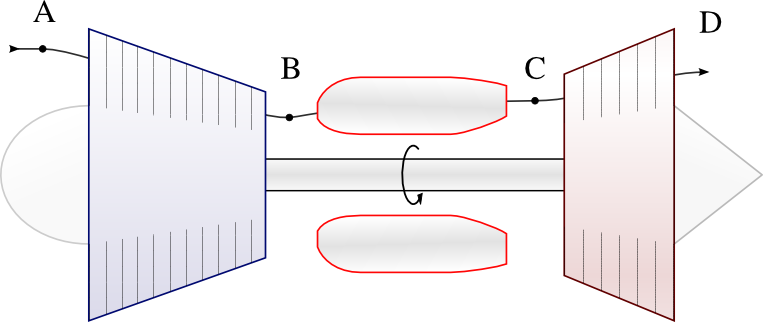
\includegraphics[scale=0.6]{images/circuit_generateur_gaz.png}\vspace{0.5cm}
				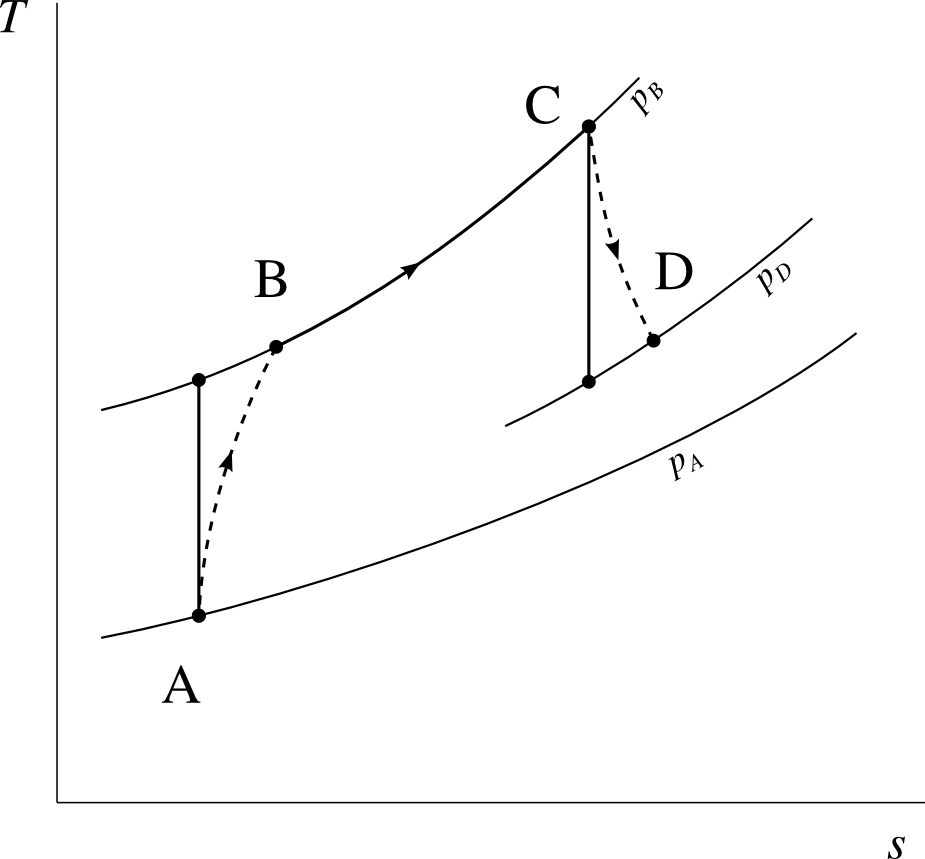
\includegraphics[scale=0.8]{images/ts_gp_generateur_gaz.png}
			\end{center}
			\supercaption{Cœur de turbomachine, ou «~générateur à gaz~» (schéma de fonctionnement et diagramme température-entropie).
			Cette installation n’a pas d’intérêt en elle-même mais a de nombreuses applications dérivées. L’une d’elles est le \vocab{turbo}, pour lequel un moteur à pistons fait office de chambre de combustion, comme décrit en \S\ref{ch_turbo}.}{schéma \ccbysa \olivier\\ diagramme \cczero \oc}
			\label{fig_générateur_gaz}
		\end{figure}

		Dans cette configuration la turbine extrait exactement assez de puissance pour alimenter le compresseur. À sa sortie, l’air est encore comprimé et peut être exploité d’une multitude de façons.



	\subsection{Turboréacteur}

		Le \vocab{turboréacteur} (\cref{fig_turboréacteur}) est la première application qui ait été faite du moteur décrit plus haut. À la sortie de la turbine, l’air est détendu dans une tuyère, ce qui l’accélère et fournit une poussée nette. C’est le fluide moteur lui-même qui est utilisé pour générer la poussée.

		\begin{figure}
		 	\begin{center}
				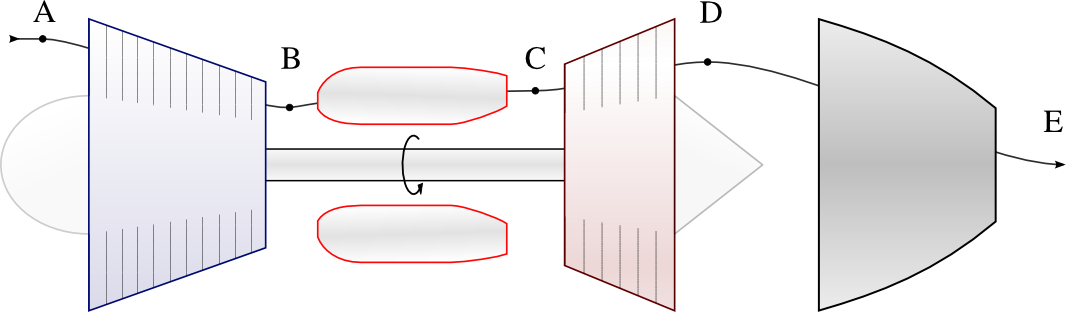
\includegraphics[scale=0.6]{images/circuit_turbojet.png}\vspace{0.5cm}
				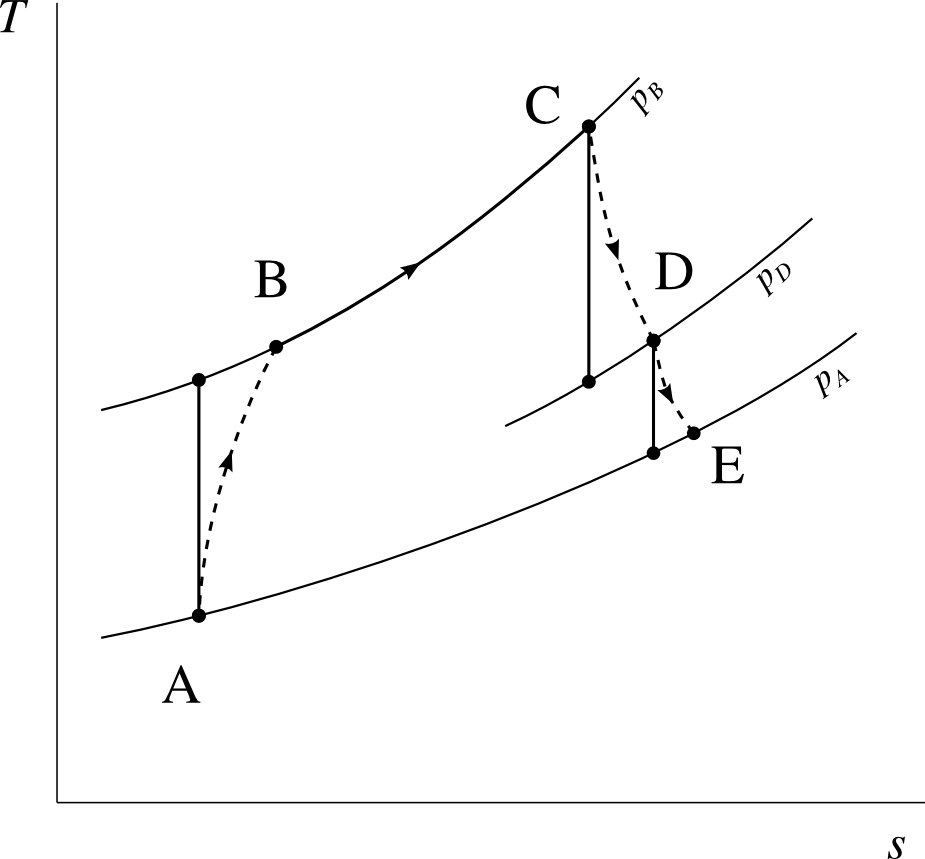
\includegraphics[scale=0.8]{images/ts_gp_turbojet.png}
			\end{center}
			\supercaption{Turboréacteur (schéma de principe et diagramme température-entropie).
			À la sortie de la turbine, l’air est encore pressurisé ; il est détendu dans une tuyère pour y être accéléré.}{schéma \ccbysa \olivier\\ diagramme \cczero \oc}
			\label{fig_turboréacteur}
		\end{figure}

		Les turboréacteurs sont extrêmement compacts et utilisés principalement sur les appareils militaires.

		 

	\subsection{Turbopropulseur et turbomoteur}
	\label{ch_turboprop_turboshaft}

		Plutôt que d’utiliser une tuyère comme dans un turboréacteur, il est possible de poursuivre la détente dans la turbine jusqu’à la pression atmosphérique. La puissance fournie par la turbine est alors \emph{supérieure} à la puissance consommée par le compresseur. 

		L’arbre moteur fournit alors du travail, que l’on peut utiliser pour alimenter une hélice propulsive (cas d’un \vocab{turbopropulseur}) ou un élément externe comme une génératrice ou une pompe (cas d’un \vocab{turbomoteur}), comme montré en \cref{fig_turbomoteur}.

		\begin{figure}
			\begin{center}
				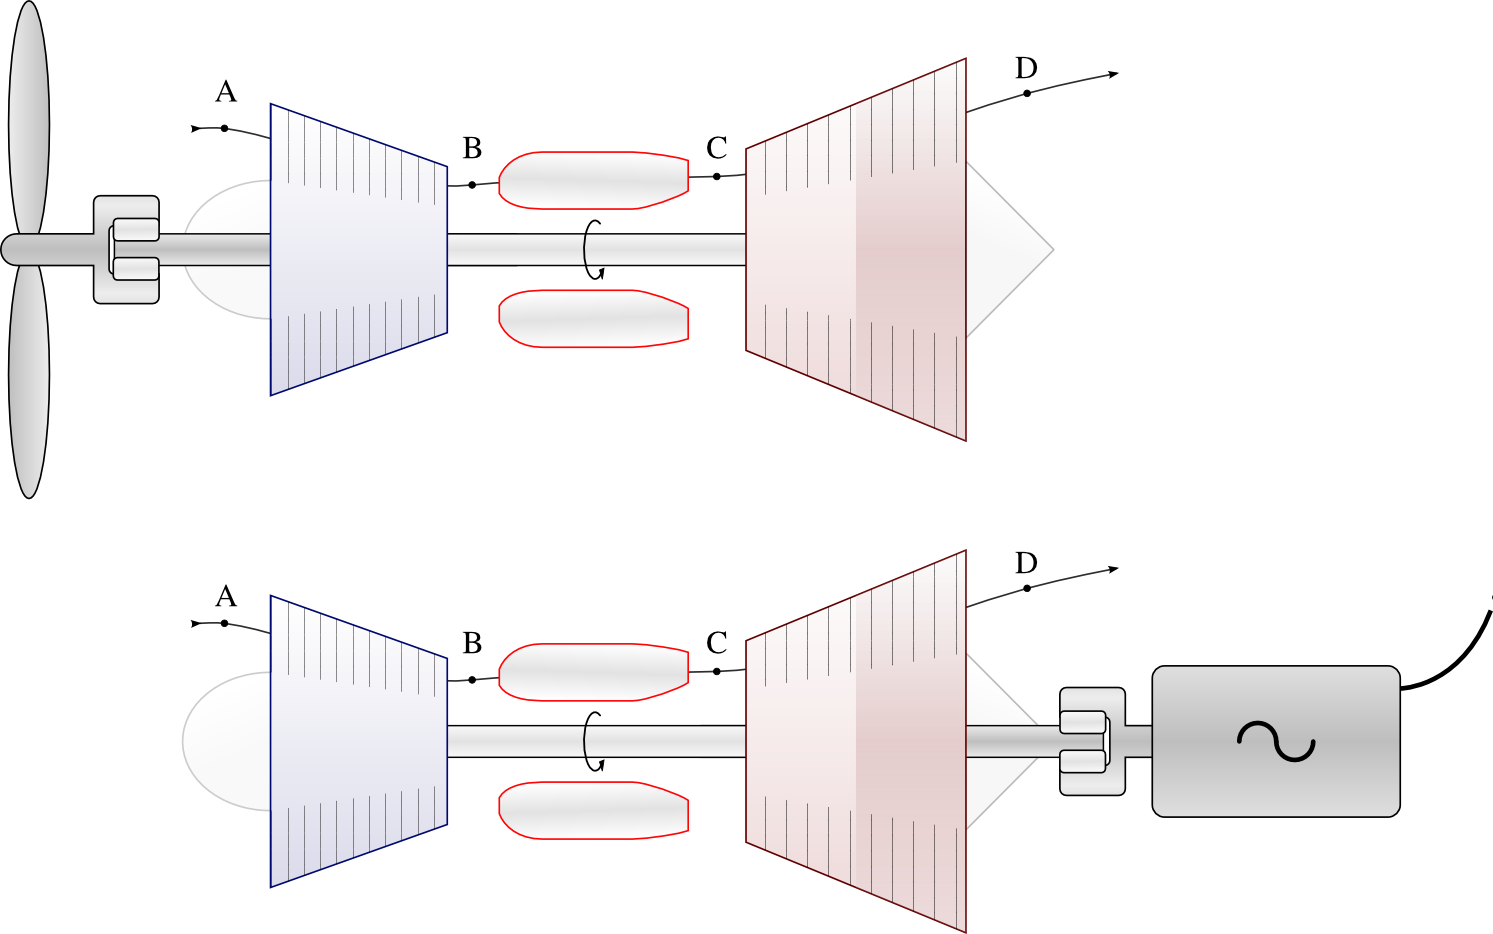
\includegraphics[scale=0.6]{images/circuit_turboprop_generateur.png}\vspace{0.5cm}
				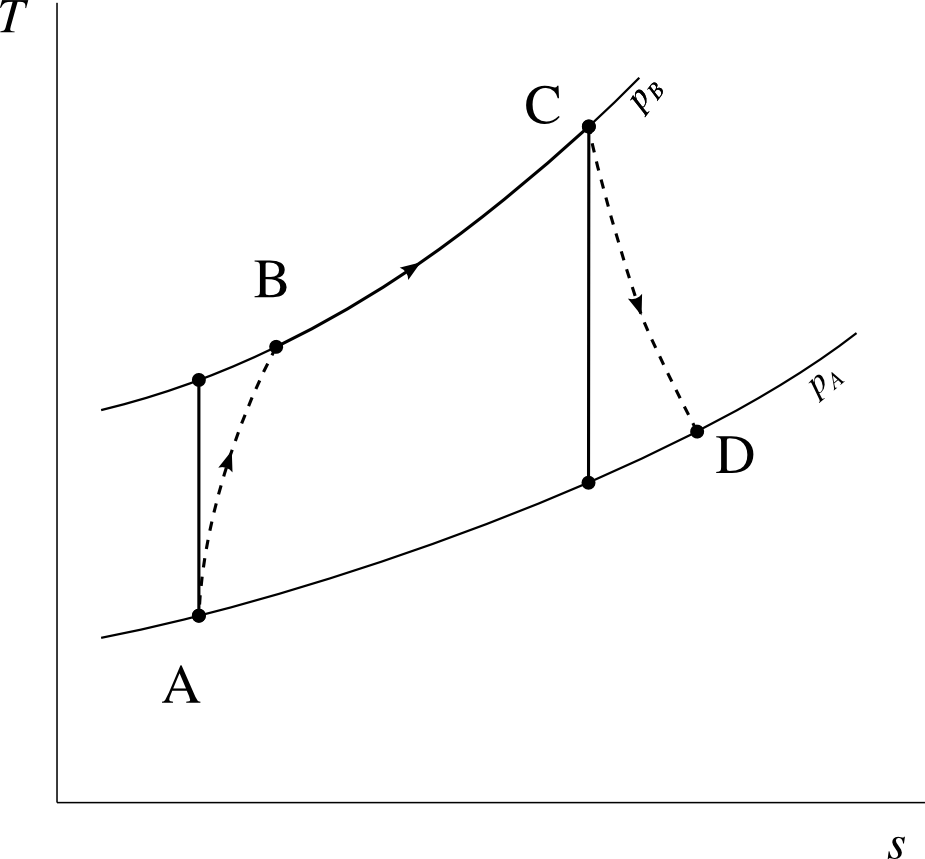
\includegraphics[scale=0.8]{images/ts_gp_turboprop_generateur.png}
			\end{center}
			\supercaption{Schémas de principe et diagramme température-entropie d’un turbopropulseur (haut) et d’un turbomoteur (bas). La puissance extraite de la turbine dépasse celle consommée par le compresseur et est utilisée pour alimenter l’hélice ou bien une génératrice.}{schémas \ccbysa \olivier\\ diagramme \cczero \oc}
			\label{fig_turbomoteur}
		\end{figure}

		L’alimentation d’une hélice de turbopropulseur, ou de la soufflante d’un turbofan, présente des avantages considérables en efficacité de propulsion que l’étudiant/e pourra étudier lors d’un cours de propulsion aéronautique. Les désavantages associés sont bien sûr l’encombrement et le poids : le diamètre des hélices et soufflantes dépasse souvent trois mètres et elles imposent de grandes contraintes structurelles et mécaniques sur le moteur.

		Les turbomoteurs, quant à eux, ont de multiples applications (hélicoptères, navires militaires, générateurs électriques d’appoint, centrales génératrices à gaz…). Ils sont plus souvent déclinés dans les variantes détaillées plus bas.


	\subsection{Turbofan}

		D’un point de vue thermodynamique, un \vocab{turbofan}\footnote{Un turbofan est parfois nommé \vocab{turboréacteur à soufflante} ou \vocab{à double flux}.} (\cref{fig_turbofan}), est équivalent à un turbopropulseur caréné, c’est-à-dire autour duquel on aurait placé un fuselage (nommé carène).
		
		\begin{figure}
			\begin{center}
				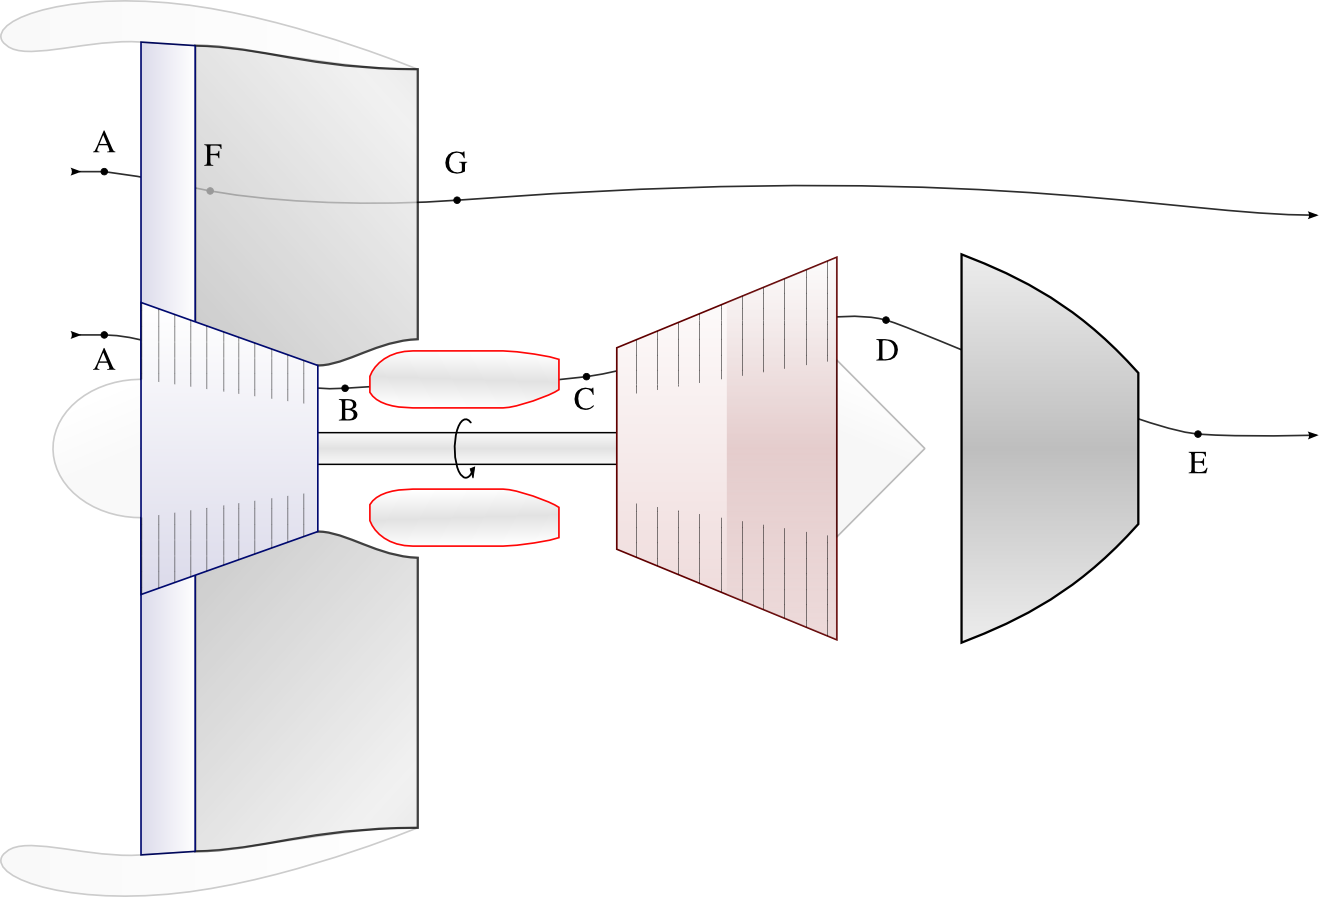
\includegraphics[scale=0.6]{images/circuit_turbofan.png}
			\end{center}
			\supercaption{Schéma de principe d’un turbofan. 
			Le circuit central du moteur ($\A \to E$) alimente mécaniquement la soufflante, qui permet au circuit externe ($\A \to G$) de fournir la majorité de la poussée.}{schéma \ccbysa \olivier}
			\label{fig_turbofan}
		\end{figure}
		
		Il y a deux flux d’air séparés au sein d’un turbofan :

		\begin{itemize}
			\item le flux central, dit parfois «~flux chaud~», est le flux du moteur proprement dit. Après combustion, il traverse une turbine dont la puissance excède largement celle du compresseur. Cet excès de puissance est transmis à la soufflante ;
			\item le flux externe, dit parfois «~flux froid~», est faiblement compressé par la soufflante et directement détendu dans la tuyère qui englobe le corps chaud du moteur. Il n’est jamais chauffé.\\
			C’est cet air «~froid~» qui fournit la plus grande part de la poussée. On montre que plus le rapport air froid / air chaud, (nommé \vocab{taux de dilution}) est grand, plus le moteur est efficace. Le taux de dilution des moteurs modernes avoisine \num{10}.
		\end{itemize}
		 

	\subsection{Turbine libre et turbines multiples}

		En fonction des applications, plusieurs agencements de turbines et compresseurs peuvent être utilisés.

		Avec une configuration à \vocab{turbine libre}, la puissance mécanique fournie par le moteur est transmise par une turbine dédiée (\cref{fig_turbine_libre}). Cela permet de maintenir chacun des deux axes à des vitesses différentes.

		\begin{figure}
			\begin{center}
				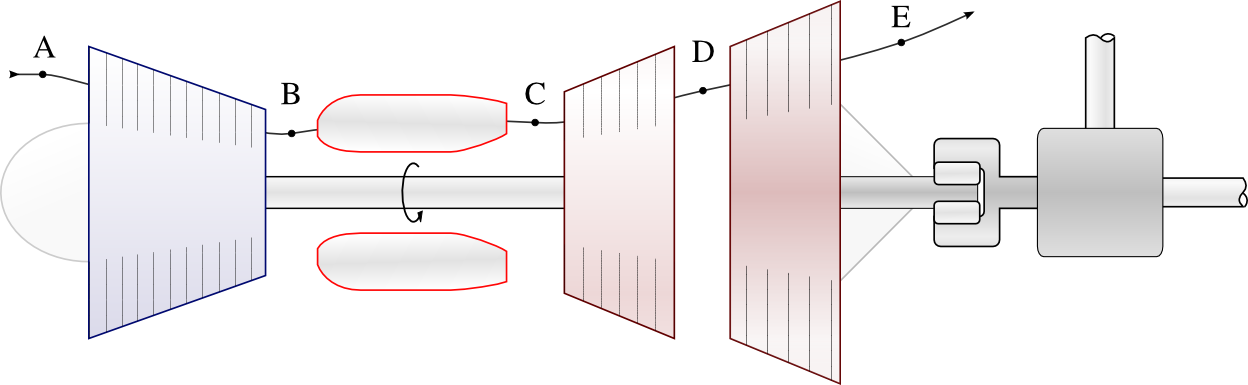
\includegraphics[scale=0.6]{images/circuit_turbine_libre.png}\vspace{0.5cm}
				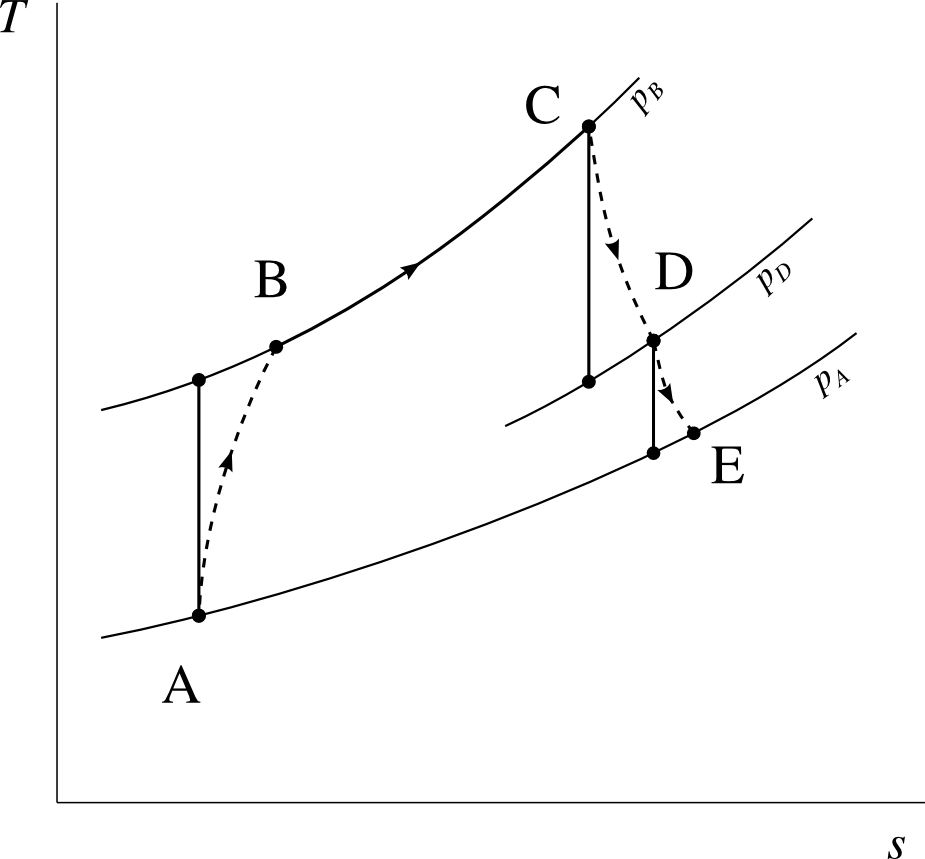
\includegraphics[scale=0.8]{images/ts_gp_turbine_libre.png}
			\end{center}
			\supercaption{Turbomoteur à turbine libre (schéma de principe et diagramme température-entropie).
			La puissance fournie par le moteur provient exclusivement de la turbine libre.}{schéma \ccbysa \olivier\\ diagramme \cczero \oc}
			\label{fig_turbine_libre}
		\end{figure}

		La vitesse de l’axe turbine/compresseur n’étant pas contrainte par la charge imposée à l’axe libre, il peut évoluer à des vitesses plus proches de son point optimum et accélérer plus aisément. Cet avantage compense la plus grande complexité mécanique de la configuration dans les applications comme la motorisation des hélicoptères, où des variations importantes de puissance sont fréquemment demandées.

		Avec une configuration à \vocab{axes multiples}, on divise compresseur et turbine en deux parties chacun, formant ainsi deux systèmes co-axiaux incorporés l’un dans l’autre (\cref{fig_axes_multiples}).

		\begin{figure}
			\begin{center}
				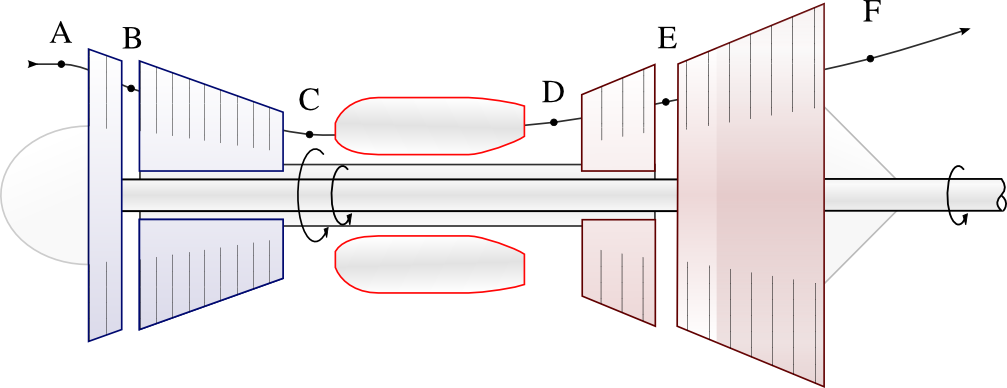
\includegraphics[scale=0.6]{images/circuit_twin_spool.png}\vspace{0.5cm}
				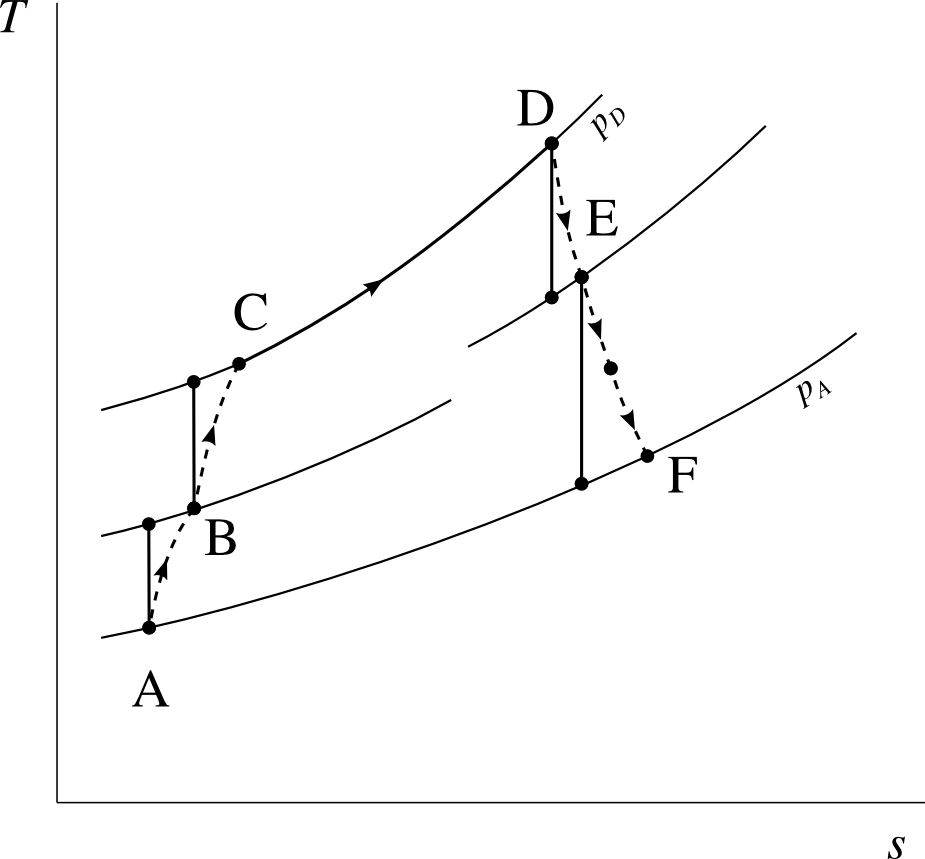
\includegraphics[scale=0.8]{images/ts_gp_twin_spool.png}
			\end{center}
			\supercaption{Turbomoteur à axes multiples (schéma de principe et diagramme température-entropie).
			Chaque axe tourne à une vitesse différente.}{schéma \ccbysa \olivier\\ diagramme \cczero \oc}
			\label{fig_axes_multiples}
		\end{figure}

		C’est la turbine haute pression qui alimente le compresseur haute pression (axe à grande vitesse), et la turbine basse pression qui alimente le compresseur basse pression (axe à faible vitesse).

		L’objectif de l’agencement est le même que pour la turbine libre : permettre à chaque axe d’évoluer à sa vitesse propre. En effet, au fur et à mesure que la pression augmente dans le compresseur, la densité et la température augmentent. Cette configuration permet de faire évoluer les pales à plus grande vitesse et réduire ainsi leur taille.




\section{Modification des cycles des turbomachines}


	\subsection{Refroidissement intermédiaire et réchauffe}
	\label{ch_intercooling}

		Pour les raisons évoquées en \S\ref{ch_criteres_evaluation_moteurs_gaz} plus haut, il est parfois souhaitable d’augmenter la marge de travail et la puissance spécifique, même au prix d’une baisse du rendement total.
		
		Pour réduire la puissance consommée par le compresseur, on a parfois recours au \vocab{refroidissement intermédiaire} (ou \vocab{intercooling}). La compression est interrompue et l’air est refroidi avant de poursuivre la compression (\cref{fig_intercooling_réchauffe}).

		\begin{figure}
			\begin{center}
				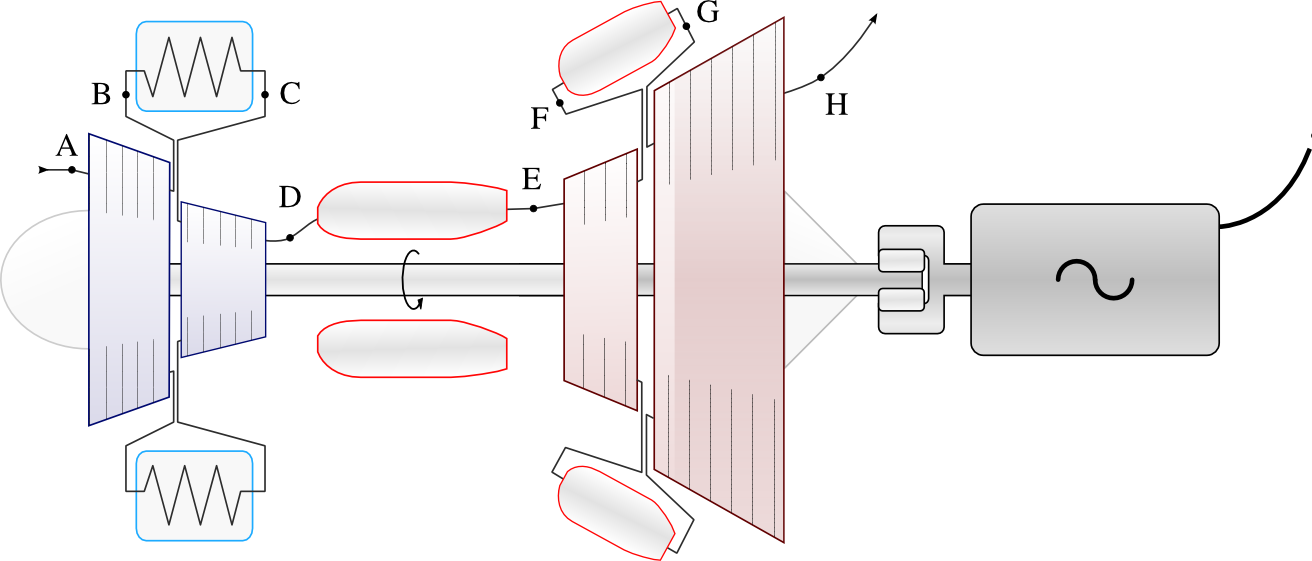
\includegraphics[scale=0.6]{images/circuit_intercooler_rechauffe.png}\vspace{1cm}
				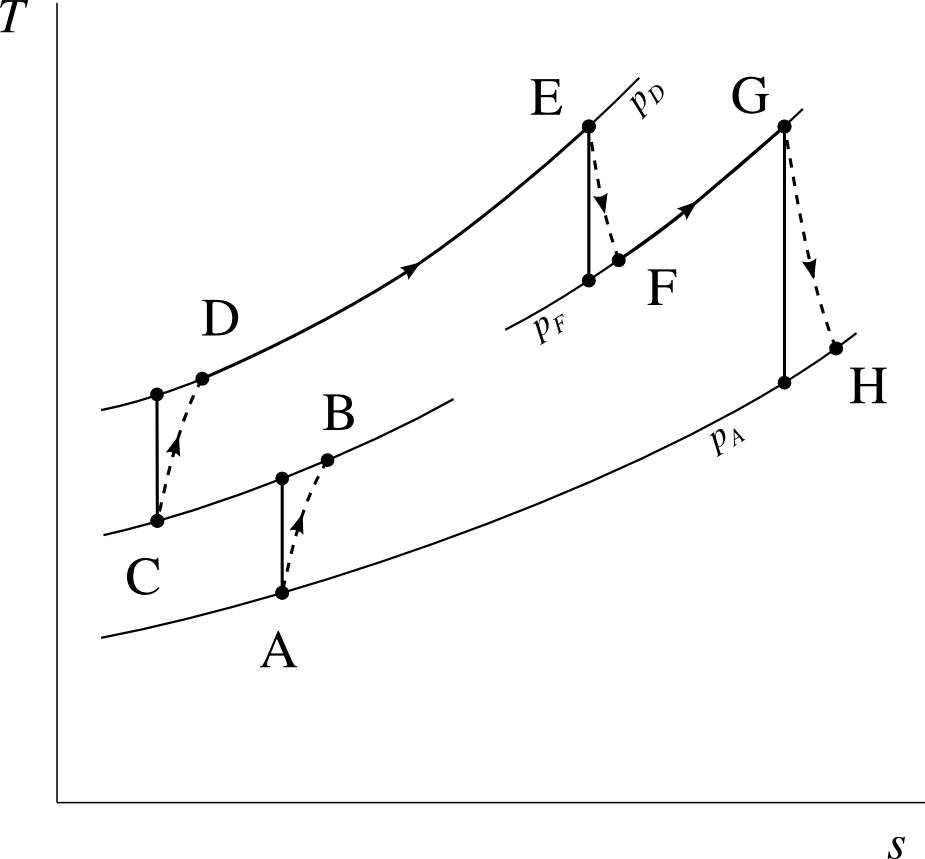
\includegraphics[scale=0.8]{images/ts_gp_intercooler_rechauffe.png}
			\end{center}
			\supercaption{Turbomoteur générateur avec refroidisseur et réchauffe (schéma de principe et diagramme température-entropie)\\
			Le refroidisseur («~\vocab{intercooler}~») refroidit l’air au milieu de sa compression ; tandis que la deuxième chambre de combustion le réchauffe au milieu de la détente. Les deux modifications sont indépendantes l’une de l’autre et peuvent être installées séparément.}{schéma \ccbysa \olivier\\ diagramme \cczero \oc}
			\label{fig_intercooling_réchauffe}
		\end{figure}

		La compression d’un gaz entre deux pressions données impose un \emph{rapport} entre les températures initiale et finale (\ref{eq_isentropique_horrible1}). Par contre, la puissance demandée pour compresser un gaz entre ces deux pressions dépend de la \emph{différence} entre ces deux températures (\ref{eq_puissance_compresseur}). Ainsi, plus la température de départ est faible, plus la puissance nécessaire pour atteindre une pression donnée sera faible.

		Dans la même optique, on peut augmenter la puissance spécifique fournie par la turbine en procédant au réchauffement des gaz avant la fin de la détente : c’est la \vocab{réchauffe}. Le principe et le procédé sont identiques à la resurchauffe des centrales à vapeur (\S\ref{ch_resurchauffe}).

		Il n’aura pas échappé à l’étudiant/e que le rendement est inévitablement réduit par l’utilisation du refroidissement intermédiaire. La chambre de combustion doit en effet fournir plus de chaleur, à température moyenne plus basse. Cette réduction du rendement fera l’objet d’un compromis avec la réduction de la taille du compresseur (usuellement la pièce la plus volumineuse d’un moteur) et l’augmentation de la puissance spécifique. Refroidissement intermédiaire et réchauffe sont caractéristiques des installations où le rapport puissance/encombrement doit être maximisé.

		Pour réduire la perte de rendement dans les moteurs au sol, il est parfois possible de récupérer de la chaleur des gaz d’échappement pour réchauffer l’air à la sortie du compresseur, et ainsi soulager la chambre de combustion à moindres frais énergétiques. L’échangeur de chaleur est parfois appelé \vocab{économiseur} (\cref{fig_intercooler_echangeur}) ; il est laissé à l’étudiant/e le loisir de retracer le cycle suivi sur un diagramme température-entropie et de retrouver les conditions nécessaires à son fonctionnement.
		
		\begin{figure}
			\begin{center}
				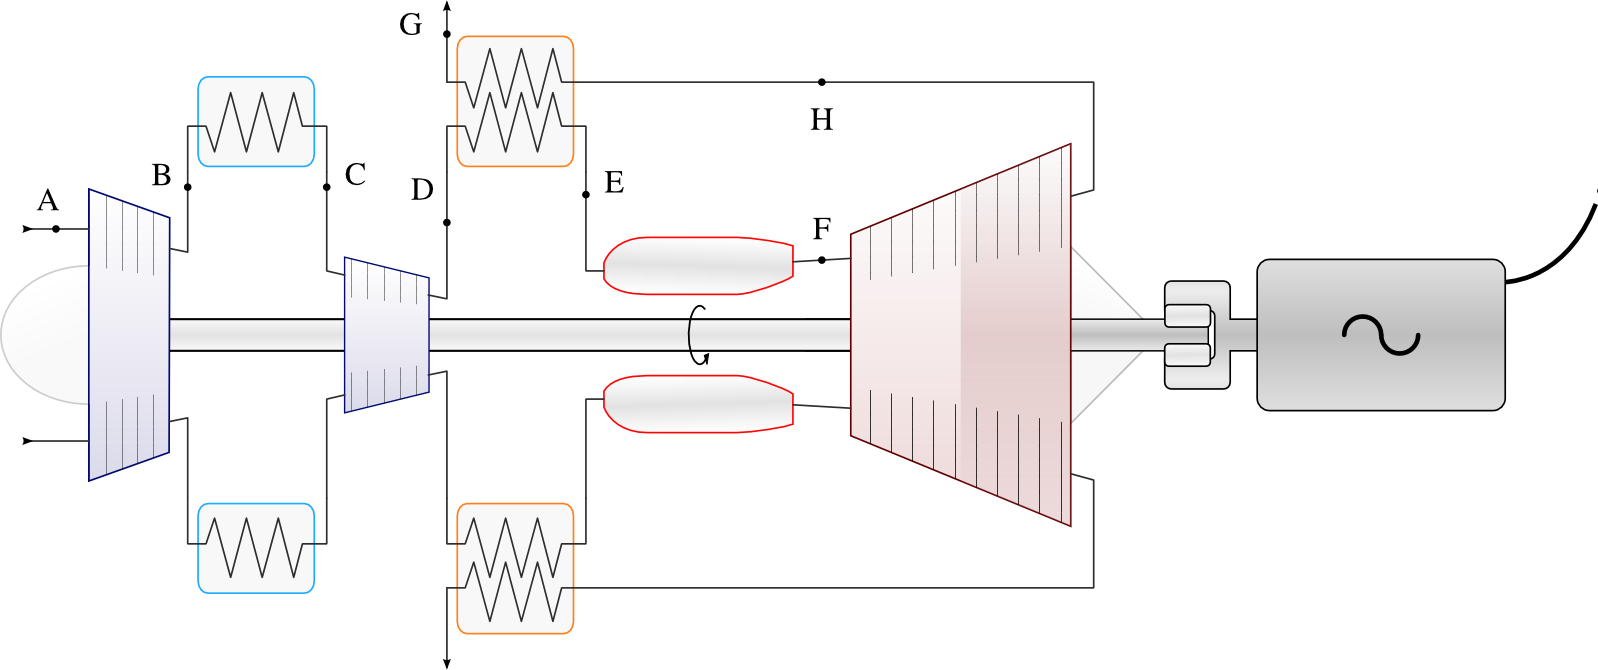
\includegraphics[scale=0.6]{images/circuit_intercooler_echangeur.png}
			\end{center}
			\supercaption{Turbomoteur générateur avec refroidisseur et échangeur économiseur (schéma de principe). Les gaz d’échappement sont redirigés vers l’intérieur du moteur pour fournir de la chaleur aux gaz à l’entrée de la chambre de combustion. Il est laissé à l’étudiant/e le soin de déterminer les limites du procédé.}{schéma \ccbysa \olivier}
			\label{fig_intercooler_echangeur}
		\end{figure}

	\subsection{Postcombustion}
	\label{ch_postcombustion}

		La \vocab{postcombustion} est l’ajout d’une seconde phase de combustion dans un turboréacteur, après la turbine et avant l’entrée dans la tuyère (\cref{fig_postcombustion}). Le principe est exactement le même que celui de la réchauffe : augmenter la poussée spécifique de la machine (au détriment de son rendement).

		\begin{figure}
			\begin{center}
				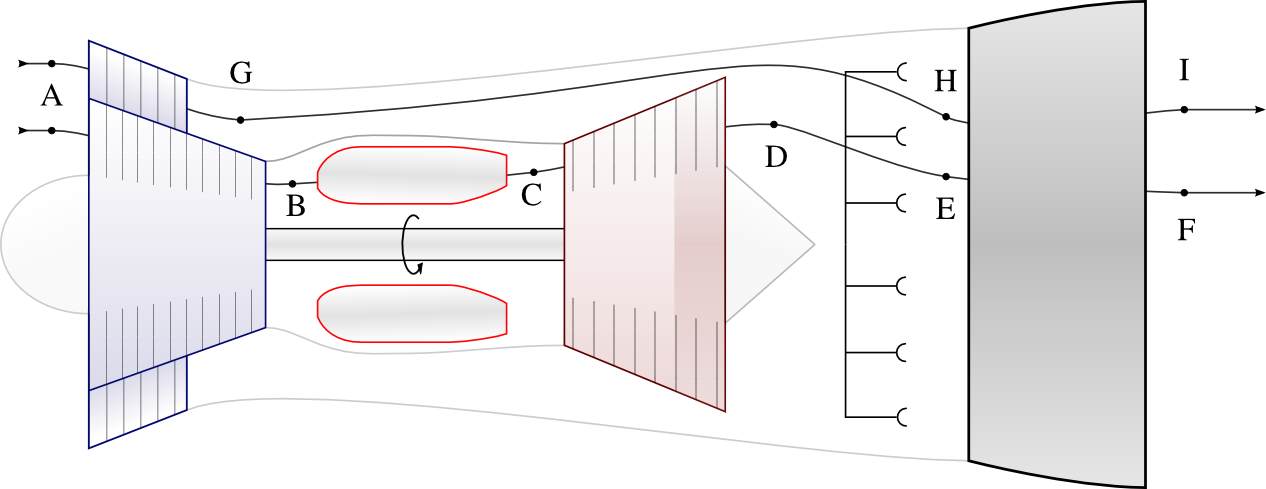
\includegraphics[scale=0.6]{images/circuit_postcombustion.png}\vspace{0.5cm}
				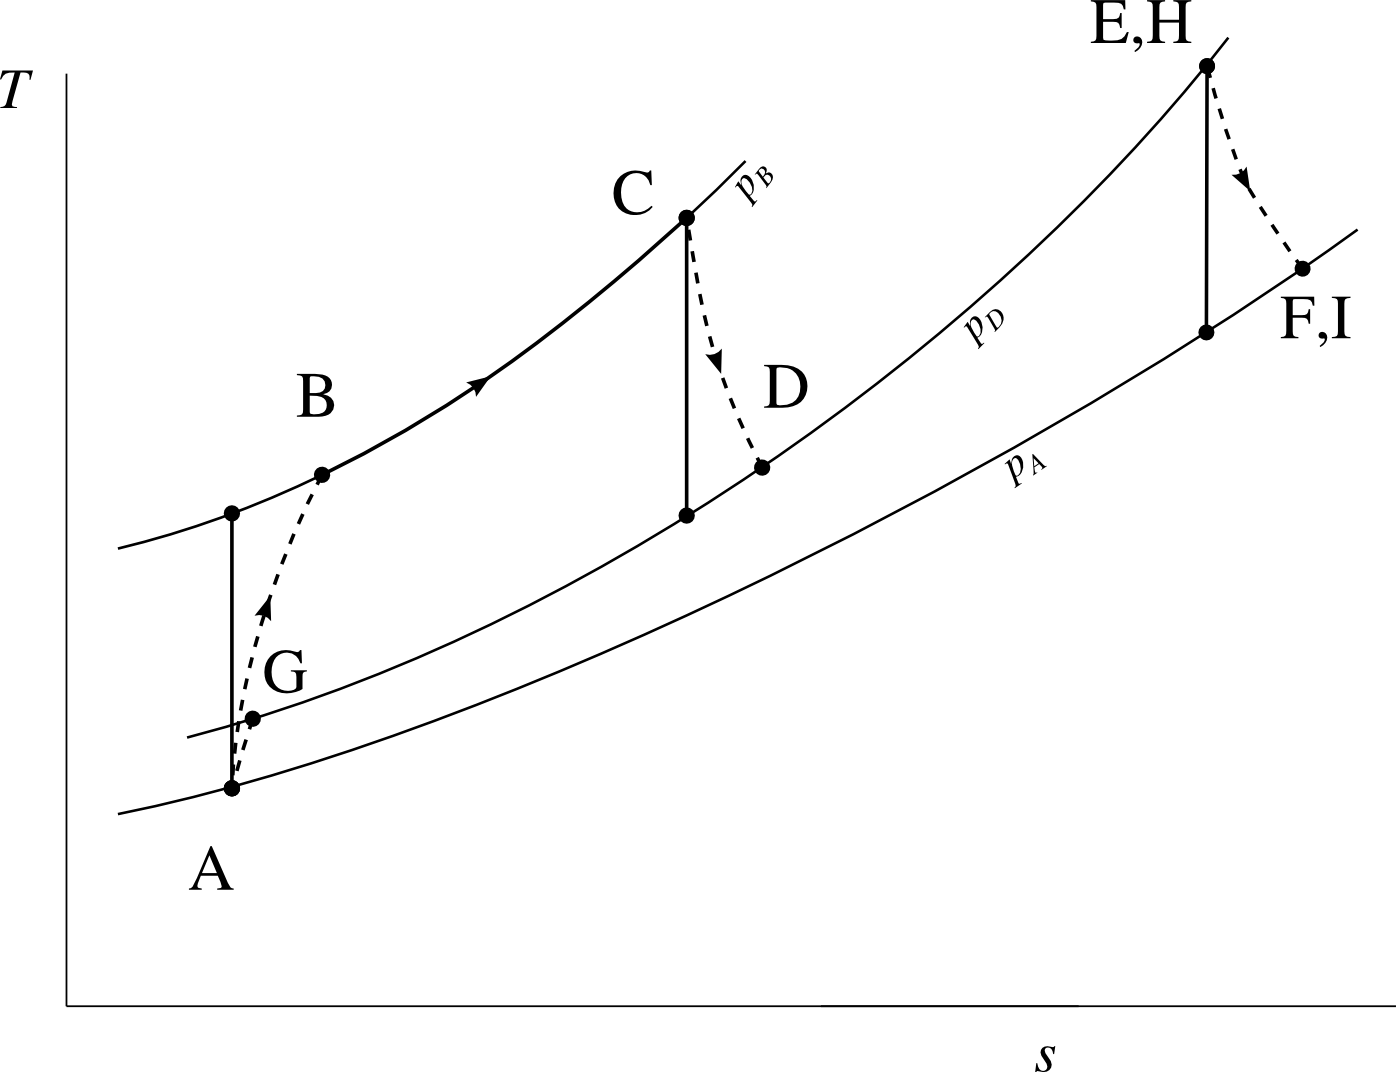
\includegraphics[scale=0.8]{images/ts_gp_postcombustion.png}
			\end{center}
			\supercaption{Postcombustion sur un turboréacteur double-flux (schéma de principe et diagramme température-entropie). Les états E et H ne sont en pratique pas nécessairement confondus.}{schéma \ccbysa \olivier\\ diagramme \cczero \oc}
			\label{fig_postcombustion}
		\end{figure}

		Tout comme la réchauffe, la postcombustion modifie les propriétés (le volume spécifique en particulier) de l’air et impose un redimensionnement des pièces en aval. La géométrie de la tuyère est ainsi modifiée en fonction de l’activation ou non de la postcombustion. L’ajout d’un système de postcombustion à un turboréacteur ne nécessite que l'installation de brûleurs ainsi que d’un système de variation de la géométrie sur la tuyère. L’augmentation du poids engendrée est faible au regard de l’augmentation de la puissance disponible.

		La perte outrageante de rendement engendrée par l’utilisation de la postcombustion, ainsi que les niveaux fracassants de bruit et de pollution qu’elle engendre, la limitent au seul domaine militaire (sur les avions de combat en particulier).

		 

	\subsection{Refroidissement de la turbine}
	\label{ch_refroidissement_turbine}

		L’augmentation du rendement et de la puissance spécifique permise par l’augmentation des températures de combustion pousse les motoristes à développer toute une série de technologies pour maximiser la température en sortie de chambre de combustion (\textsc{tet}, pour \vocab{température d’entrée de turbine}).

		Le principal stratagème employé est de refroidir la turbine avec de l’air prélevé dans le compresseur (\cref{fig_refroidissement_turbine}). L’air prélevé est conduit au travers des pales de la turbine et permet d’élever la température de combustion sans risquer d’endommager les pales. Les systèmes de refroidissement les plus efficaces et les plus avancés enrobent \emph{l’extérieur} des pales de turbine avec cet air prélevé dans compresseur. La température \textsc{tet} peut ainsi dépasser la température de fonte des pales de plus d’une centaine de degrés Celsius !

		\begin{figure}
			\begin{center}
				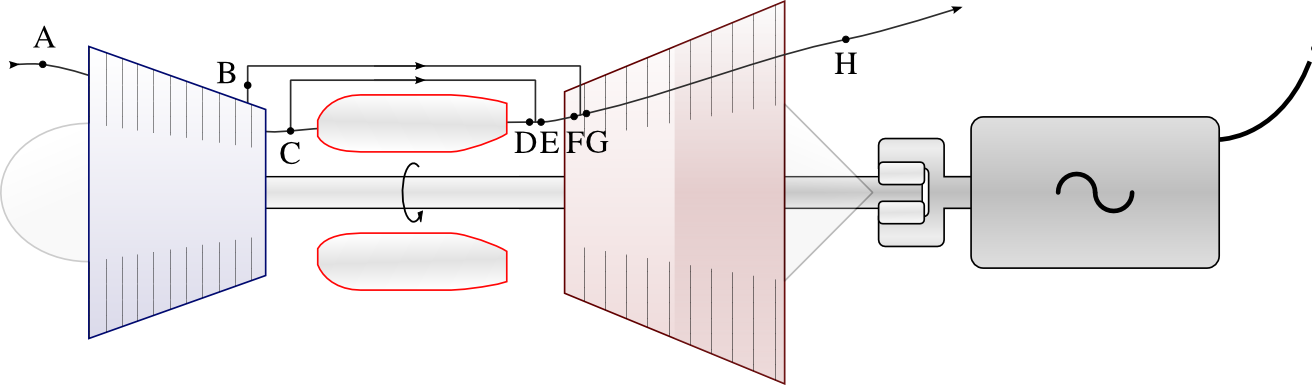
\includegraphics[scale=0.6]{images/circuit_refroidissement_turbine.png}\vspace{0.5cm}
				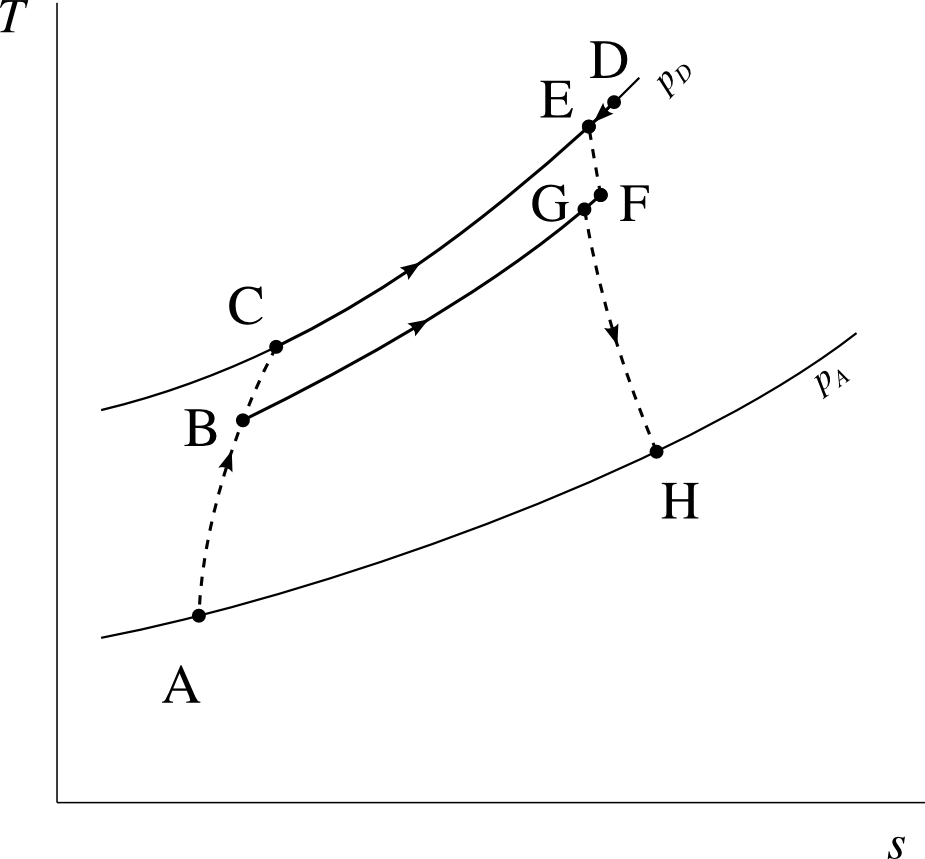
\includegraphics[scale=0.8]{images/ts_gp_refroidissement_turbine.png}
			\end{center}
			\supercaption{Refroidissement de la turbine à l’aide d’air prélevé sur le compresseur (schéma de principe et diagramme température-entropie).
			Cet air, à température modérée, contourne la chambre de combustion et n’entre jamais en contact avec le carburant. Ici le moteur représenté est un turbomoteur, mais le refroidissement turbine est utilisable sur toute configuration.}{schéma \ccbysa \olivier\\ diagramme \cczero \oc}
			\label{fig_refroidissement_turbine}
		\end{figure}

		Un tel refroidissement de la turbine a un coût conséquent. D’une part, dans un moteur réel, la détente de l’air de refroidissement dans la turbine fournit moins d’énergie que n’en consomme sa compression dans le compresseur (dans le cas limite où la compression et la détente sont isentropiques, ce coût énergétique est nul). La circulation de cet air représente donc une charge qui doit être compensée par l’augmentation de l’efficacité qu’elle engendre. D’autre part, le compresseur et la turbine doivent être surdimensionnés pour admettre un débit d’air plus grand

		Le refroidissement des turbines est un axe majeur de recherche en propulsion aéronautique. Il faut combiner de nombreux domaines technologiques (matériaux, mécanique des fluides, agencement mécanique, chimie de combustion) pour remplir ces objectifs de nature thermodynamique.

		\begin{landscape}

		\begin{figure}
			\begin{center}
				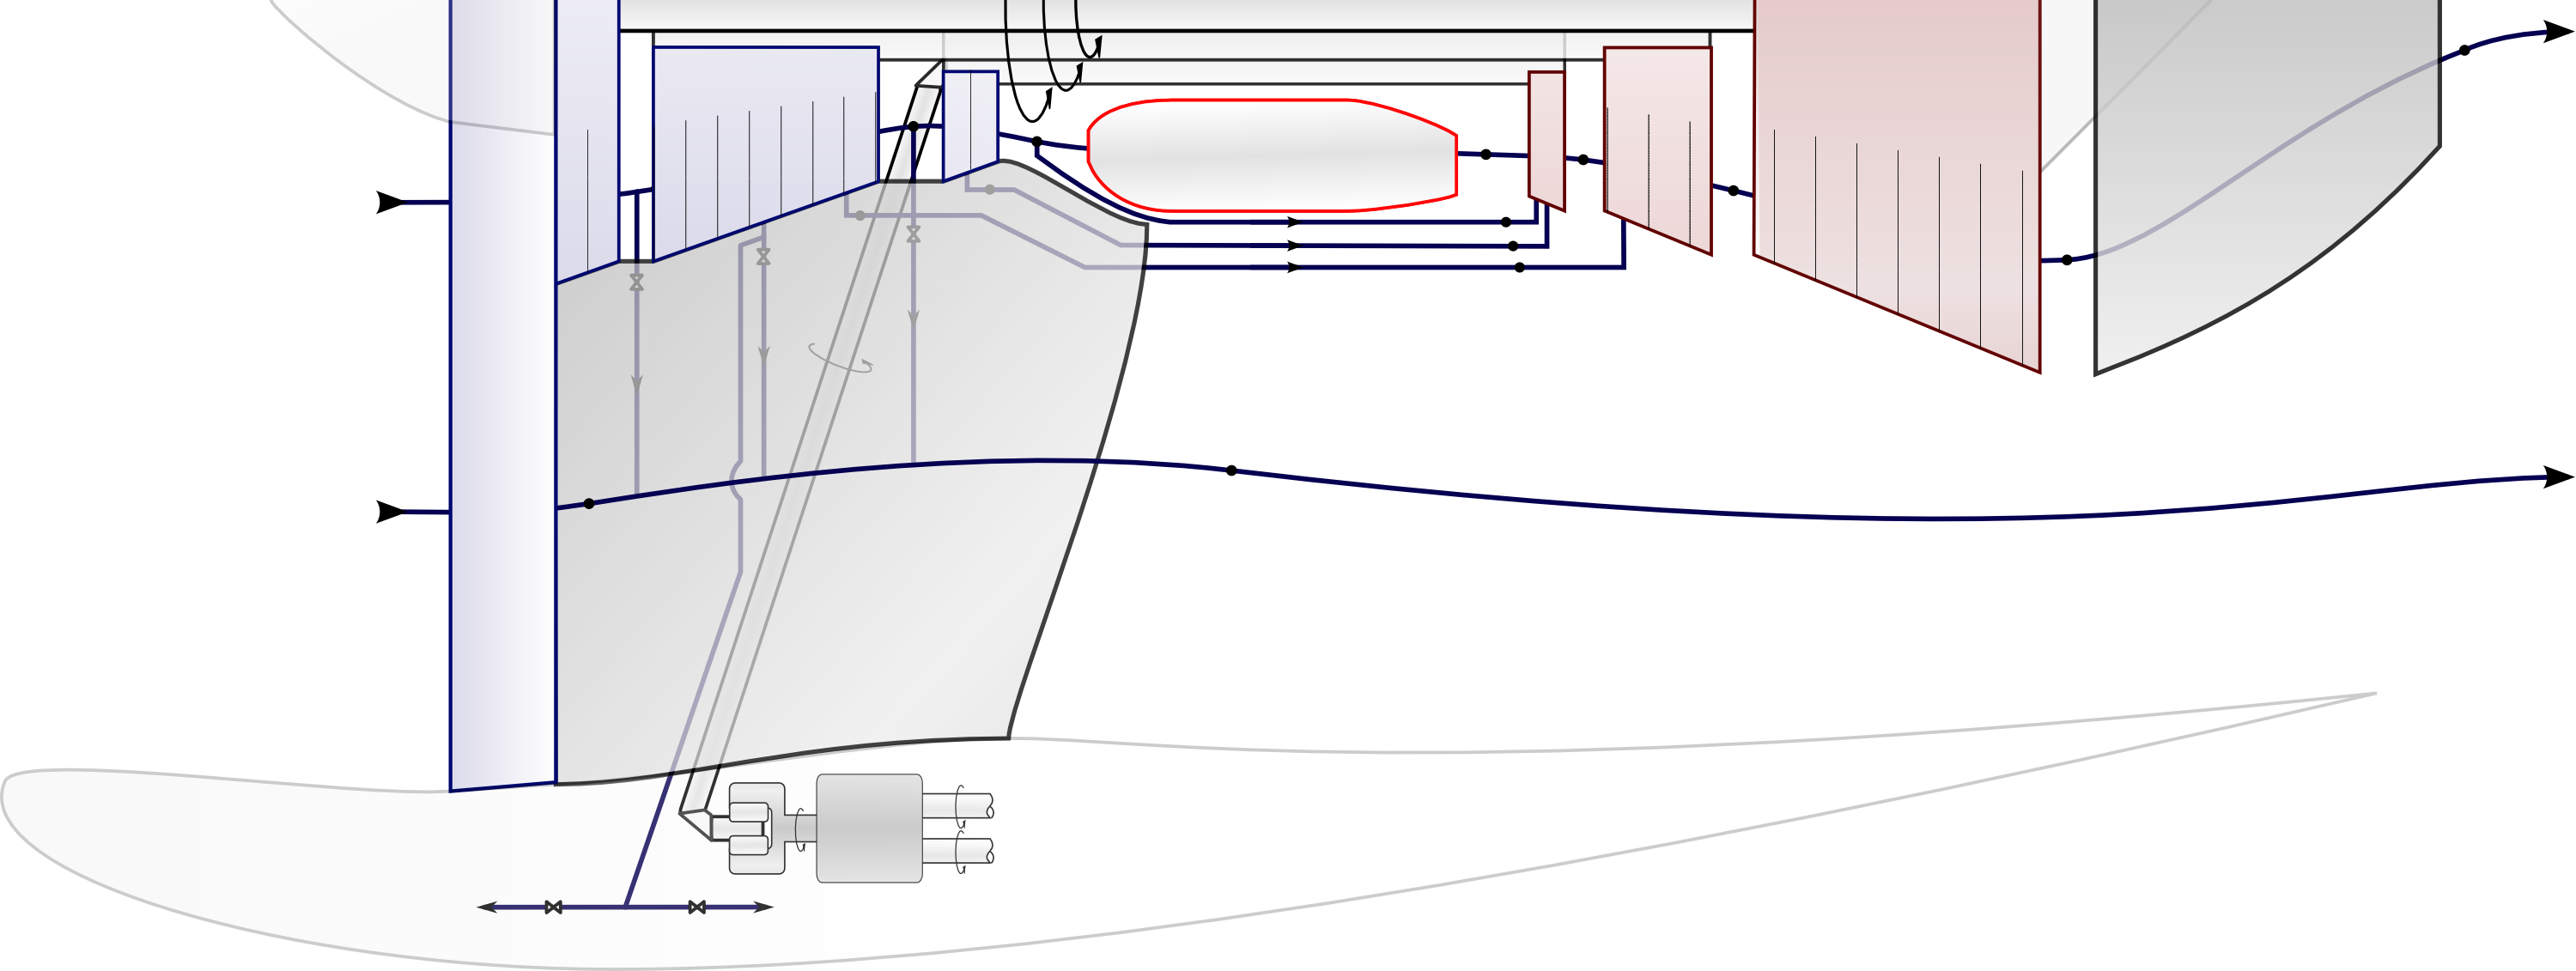
\includegraphics[width=\linewidth]{images/circuit_turbofan_complet.png}
			\end{center}
			\supercaption{Schéma du circuit thermodynamique d’un turbofan moderne.
			L’installation combine axes multiples, extractions de puissance mécanique et pneumatique, prélèvements de refroidissement turbine et deux flux d’air principaux (il est laissé encore une fois à l’étudiant/e le loisir de tracer le cycle sur un diagramme température-entropie).
			Sur les appareils bimoteurs qualifiés pour effectuer des vols \textsc{etops}, chaque moteur doit pouvoir assurer seul le vol de l’appareil et l’alimentation de nombreux systèmes (pressurisation, dégivrage, chauffage, génération électrique et pneumatique) pendant plusieurs heures avec une fiabilité démontrée.}{schéma \ccbysa \olivier}
		\end{figure}

		\end{landscape}
